% ********************************************************************
% A Classic Thesis Style
% An Homage to The Elements of Typographic Style
%
% Copyright (C) 2018 André Miede and Ivo Pletikosić
%
% If you like the style then I would appreciate a postcard. My address
% can be found in the file ClassicThesis.pdf. A collection of the
% postcards I received so far is available online at
% http://postcards.miede.de
%
% License:
% This program is free software; you can redistribute it and/or modify
% it under the terms of the GNU General Public License as published by
% the Free Software Foundation; either version 2 of the License, or
% (at your option) any later version.
%
% This program is distributed in the hope that it will be useful,
% but WITHOUT ANY WARRANTY; without even the implied warranty of
% MERCHANTABILITY or FITNESS FOR A PARTICULAR PURPOSE.  See the
% GNU General Public License for more details.
%
% You should have received a copy of the GNU General Public License
% along with this program; see the file COPYING.  If not, write to
% the Free Software Foundation, Inc., 59 Temple Place - Suite 330,
% Boston, MA 02111-1307, USA.
%
% PLEASE SEE ALSO THE AUTHORS' NOTE REGARDING THIS LICENSE
% IN THE DOCUMENTATION (ClassicThesis.pdf --> Chapter 1 / Chapter01.tex)
% ********************************************************************
\RequirePackage{silence} % :-\
    \WarningFilter{scrreprt}{Usage of package `titlesec'}
    %\WarningFilter{scrreprt}{Activating an ugly workaround}
    \WarningFilter{titlesec}{Non standard sectioning command detected}
\documentclass[ oneside,openright,titlepage,numbers=noenddot,%1headlines,
                headinclude,footinclude,cleardoublepage=empty,abstract=on,
                BCOR=5mm,paper=a4,fontsize=11pt
                ]{report}
\usepackage[a4paper,
            bindingoffset=0.2in,
            left=1in,
            right=1in,
            top=1in,
            bottom=1in,
            footskip=.25in]{geometry}


%----------------------------------------------------------------------------------------
%	INPUT CONFIGURATION
%----------------------------------------------------------------------------------------
%----------------------------------------------------------------------------------------
%	CHAR ENCODING
%----------------------------------------------------------------------------------------
% 0. Set the encoding of your files. UTF-8 is the only sensible encoding nowadays. If you
% can't read äöüßáéçèê∂åëæƒÏ€ then change the encoding setting in your editor, not the line 
% below. If your editor does not support utf8 use another editor!

\PassOptionsToPackage{utf8}{inputenc}
  \usepackage{inputenc}

\PassOptionsToPackage{T1}{fontenc} % T2A for cyrillics
  \usepackage{fontenc}


%----------------------------------------------------------------------------------------
%	CONFIGURATION
%----------------------------------------------------------------------------------------
% 1. Configure classicthesis for your needs here, e.g., remove "drafting" below
% in order to deactivate the time-stamp on the pages

\PassOptionsToPackage{
  drafting=false,           % print version information on the bottom of the pages
  tocaligned=false,         % the left column of the toc will be aligned (no indentation)
  dottedtoc=true,           % page numbers in ToC flushed right
  eulerchapternumbers=true, % use AMS Euler for chapter font (otherwise Palatino)
  linedheaders=false,       % chaper headers will have line above and beneath
  floatperchapter=true,     % numbering per chapter for all floats (i.e., Figure 1.1)
  eulermath=false,          % use awesome Euler fonts for mathematical formulae (pdfLaTeX)
  beramono=true,            % toggle a nice monospaced font (w/ bold)
  palatino=true,            % deactivate standard font for loading another one, see the last 
                            % section at the end of this file for suggestions
  style=arsclassica         % classicthesis, arsclassica
}{classicthesis}

%----------------------------------------------------------------------------------------
%	PERSONAL DATA AND USER AD-HOC COMMANDS
%----------------------------------------------------------------------------------------
%\newcommand{\myTitle}{Title\xspace}
\newcommand{\myTitle}{Methoden der Analyse von Sozialen Netzwerken\xspace}
\newcommand{\mySubtitle}{Bachelor Thesis\xspace}
\newcommand{\myDegree}{Bachelor of Science\xspace}
\newcommand{\myName}{Tanja \& Zast\xspace}
\newcommand{\myProf}{Prof. Dr.-Ing. Dr. h.c. Stefan Wesner\xspace}
\newcommand{\myOtherProf}{Dr. Dipl.-Inf. Lutz Schubert\xspace}
\newcommand{\myFaculty}{Faculty of Engineering, Computer Science and Psychology\xspace}
\newcommand{\myDepartment}{Institute of Information Resource Management\xspace}
\newcommand{\myUni}{Ulm University\xspace}
\newcommand{\myLocation}{Ulm\xspace}
\newcommand{\myTime}{Februar 2022\xspace}
\newcommand{\myVersion}{\classicthesis}

%----------------------------------------------------------------------------------------
%	SETUP & FINE-TUNING
%----------------------------------------------------------------------------------------
\providecommand{\mLyX}{L\kern-.1667em\lower.25em\hbox{Y}\kern-.125emX\@}
\newcommand{\ie}{i.\,e.}
\newcommand{\Ie}{I.\,e.}
\newcommand{\eg}{e.\,g.}
\newcommand{\Eg}{E.\,g.}


%----------------------------------------------------------------------------------------
%	PACKAGES
%----------------------------------------------------------------------------------------
\PassOptionsToPackage{ngerman,american}{babel} % change this to your language(s), main language last
% Spanish languages need extra options in order to work with this template
%\PassOptionsToPackage{spanish,es-lcroman}{babel}
    \usepackage{babel}

\usepackage{csquotes}
\PassOptionsToPackage{%
  %backend=biber,bibencoding=utf8, %instead of bibtex
  backend=bibtex8,bibencoding=ascii,%
  language=auto,%
  style=numeric-comp,%
  %style=authoryear-comp, % Author 1999, 2010
  %bibstyle=authoryear,dashed=false, % dashed: substitute rep. author with ---
  sorting=nyt, % name, year, title
  maxbibnames=10, % default: 3, et al.
  %backref=true,%
  natbib=true % natbib compatibility mode (\citep and \citet still work)
}{biblatex}
    \usepackage{biblatex}

\PassOptionsToPackage{fleqn}{amsmath}       % math environments and more by the AMS
  \usepackage{amsmath}

%----------------------------------------------------------------------------------------
%	GENERAL USEFUL PACKAGES
%----------------------------------------------------------------------------------------
\usepackage{graphicx} %
\usepackage{scrhack} % fix warnings when using KOMA with listings package
\usepackage{xspace} % to get the spacing after macros right
\PassOptionsToPackage{printonlyused, smaller, withpage}{acronym}
  \usepackage{acronym} % nice macros for handling all acronyms in the thesis
  %\renewcommand{\bflabel}[1]{{#1}\hfill} % fix the list of acronyms --> no longer working
  %\renewcommand*{\acsfont}[1]{\textsc{#1}}
  %\renewcommand*{\aclabelfont}[1]{\acsfont{#1}}
  %\def\bflabel#1{{#1\hfill}}
  \def\bflabel#1{{\acsfont{#1}\hfill}}
  \def\aclabelfont#1{\acsfont{#1}}


%\usepackage{pgfplots} % External TikZ/PGF support (thanks to Andreas Nautsch)
%\usetikzlibrary{external}
%\tikzexternalize[mode=list and make, prefix=ext-tikz/]


%----------------------------------------------------------------------------------------
%	TABLES, (SUB)FIGURES, AND CAPTIONS
%----------------------------------------------------------------------------------------
\usepackage{tabularx} % better tables
  \setlength{\extrarowheight}{3pt} % increase table row height
\newcommand{\tableheadline}[1]{\multicolumn{1}{l}{\spacedlowsmallcaps{#1}}}
\newcommand{\myfloatalign}{\centering} % to be used with each float for alignment
% \usepackage{subfig}
%\usepackage{todonotes}
\usepackage{pdflscape}
\usepackage{caption}
\usepackage{subcaption}
\usepackage{placeins}


%----------------------------------------------------------------------------------------
%	CODE LISTINGS
%----------------------------------------------------------------------------------------
\usepackage{listings}
%\lstset{emph={trueIndex,root},emphstyle=\color{BlueViolet}}%\underbar} % for special keywords
\lstset{language=[LaTeX]Tex,%C++,
  morekeywords={PassOptionsToPackage,selectlanguage},
  keywordstyle=\color{RoyalBlue},%\bfseries,
  basicstyle=\small\ttfamily,
  %identifierstyle=\color{NavyBlue},
  commentstyle=\color{Green}\ttfamily,
  stringstyle=\rmfamily,
  numbers=none,%left,%
  numberstyle=\scriptsize,%\tiny
  stepnumber=5,
  numbersep=8pt,
  showstringspaces=false,
  breaklines=true,
  %frameround=ftff,
  %frame=single,
  belowcaptionskip=.75\baselineskip
  %frame=L
}

%----------------------------------------------------------------------------------------
%	MAIN PACKAGE
%----------------------------------------------------------------------------------------
\usepackage{classicthesis}

%----------------------------------------------------------------------------------------
%	HYPERREFERENCES (hyperref should be called last)
%----------------------------------------------------------------------------------------
\hypersetup{%
  %draft, % hyperref's draft mode, for printing see below
  colorlinks=true, linktocpage=true, pdfstartpage=3, pdfstartview=FitV,%
  % uncomment the following line if you want to have black links (e.g., for printing)
  %colorlinks=false, linktocpage=false, pdfstartpage=3, pdfstartview=FitV, pdfborder={0 0 0},%
  breaklinks=true, pageanchor=true,%
  pdfpagemode=UseNone, %
  % pdfpagemode=UseOutlines,%
  plainpages=false, bookmarksnumbered, bookmarksopen=true, bookmarksopenlevel=1,%
  hypertexnames=true, pdfhighlight=/O,%nesting=true,%frenchlinks,%
  urlcolor=CTurl, linkcolor=CTurl, citecolor=CTurl, %pagecolor=RoyalBlue,%
  %urlcolor=Black, linkcolor=Black, citecolor=Black, %pagecolor=Black,%
  pdftitle={\myTitle},%
  pdfauthor={\textcopyright\ \myName, \myUni, \myFaculty},%
  pdfsubject={},%
  pdfkeywords={},%
  pdfcreator={pdfLaTeX},%
  pdfproducer={LaTeX with hyperref and classicthesis}%
}

%----------------------------------------------------------------------------------------
%	AUTOREFERENCES
%----------------------------------------------------------------------------------------
% There are some issues regarding autorefnames
% http://www.tex.ac.uk/cgi-bin/texfaq2html?label=latexwords
% you have to redefine the macros for the
% language you use, e.g., american, ngerman
% (as chosen when loading babel/AtBeginDocument)

\makeatletter
\@ifpackageloaded{babel}%
  {%
    \addto\extrasamerican{%
      \renewcommand*{\figureautorefname}{Figure}%
      \renewcommand*{\tableautorefname}{Table}%
      \renewcommand*{\partautorefname}{Part}%
      \renewcommand*{\chapterautorefname}{Chapter}%
      \renewcommand*{\sectionautorefname}{Section}%
      \renewcommand*{\subsectionautorefname}{Section}%
      \renewcommand*{\subsubsectionautorefname}{Section}%
    }%
    \addto\extrasngerman{%
      \renewcommand*{\paragraphautorefname}{Absatz}%
      \renewcommand*{\subparagraphautorefname}{Unterabsatz}%
      \renewcommand*{\footnoteautorefname}{Fu\"snote}%
      \renewcommand*{\FancyVerbLineautorefname}{Zeile}%
      \renewcommand*{\theoremautorefname}{Theorem}%
      \renewcommand*{\appendixautorefname}{Anhang}%
      \renewcommand*{\equationautorefname}{Gleichung}%
      \renewcommand*{\itemautorefname}{Punkt}%
    }%
      % Fix to getting autorefs for subfigures right (thanks to Belinda Vogt for changing the definition)
      \providecommand{\subfigureautorefname}{\figureautorefname}%
    }{\relax}
\makeatother


%----------------------------------------------------------------------------------------
%	BIBLIOGRAPHIES
%----------------------------------------------------------------------------------------
\addbibresource{Bibliography/Bibliography.bib}
\addbibresource[label=ownpubs]{Bibliography/AMiede_Publications.bib}

%----------------------------------------------------------------------------------------
%	HYPHENATION
%----------------------------------------------------------------------------------------
%\hyphenation{put special hyphenation here}

%----------------------------------------------------------------------------------------
%	BEGIN DOCUMENT
%----------------------------------------------------------------------------------------
\begin{document}

\newgeometry
\frenchspacing
\raggedbottom
\selectlanguage{ngerman} % american ngerman
%\renewcommand*{\bibname}{new name}
%\setbibpreamble{}
\pagenumbering{roman}
\pagestyle{plain}

%----------------------------------------------------------------------------------------
%	FRONTMATTER
%----------------------------------------------------------------------------------------
%----------------------------------------------------------------------------------------
%	LITTLE DIRTY TITLEPAGE
%----------------------------------------------------------------------------------------
\thispagestyle{empty}

%----------------------------------------------------------------------------------------
%	NAME AND TITLE
%----------------------------------------------------------------------------------------
\begin{center}
    \spacedlowsmallcaps{\myName} \\ \medskip

    \begingroup
        \color{CTtitle}\spacedallcaps{\myTitle\\
        \footnotesize{(\mySubtitle)}}
    \endgroup
\end{center}

%----------------------------------------------------------------------------------------
%	TITLEPAGE

%\begin{titlepage}
%    %\pdfbookmark[1]{\myTitle}{titlepage}
%    \begin{addmargin}[-1cm]{-3cm}
%    \begin{center}
%        \hfill
%        \vfill
%        
%        
\includegraphics[width=3cm]{Graphics/omi_logo.pdf}
%        \hfill
%        
\includegraphics[width=7.3cm]{Graphics/uulm_logo.pdf} \\ \bigskip
%        \vfill
%        
%        \noindent\rule{\linewidth}{0.4pt} \\
%        \vspace{2em}
%        \begingroup
%            \color{CTtitle}\spacedallcaps{\myTitle} \\ \bigskip
%        \endgroup
%        \noindent\rule{\linewidth}{0.4pt} \\
%        \spacedlowsmallcaps{\myName}
%        
%        \vfill
%
%        \mySubtitle \\ \medskip
%        %\myDegree \\
%        \myDepartment \\
%        \myFaculty \\
%        \myUni \\ \bigskip
%        \myTime\ %-- \myVersion
%        
%        \vspace{3em}
%        
%        \myProf \\
%        \myOtherProf \\ \medskip
%        \mySupervisor
%        \vfill
%    \end{center}
%  \end{addmargin}
%\end{titlepage}


\begin{titlepage}
    %\pdfbookmark[1]{\myTitle}{titlepage}
    \begin{addmargin*}
    \begin{center}
        %\hfill
        %\vfill
        
        \hfill
        
\includegraphics[width=7.3cm]{Graphics/uulm_logo.pdf} \\ \bigskip
        \vfill

        \noindent\rule{\linewidth}{0.4pt} \\
        \vspace{2em}
        \begingroup
            \color{CTtitle}\spacedallcaps{\myTitle} \\ \bigskip
        \endgroup
        \noindent\rule{\linewidth}{0.4pt} \\
        \spacedlowsmallcaps{\myName \myDegree} 
        \vspace{3em}
        
        \mySubtitle \\ \medskip   
        \vfill
        
        
\includegraphics[width=2.5cm]{Graphics/omi_logo.pdf}
        \vspace{1em}
        
        \myDepartment \\
        \myFaculty \\
        \myUni \\ \bigskip
        \myTime\ %-- \myVersion
        
        \vspace{3em}
        
        \myProf \\
        \myOtherProf \\ \medskip
        \vfill
    \end{center}
    \noindent\myName: \textit{\myTitle,} \mySubtitle, %\myDegree,
\textcopyright\ \myTime
  \end{addmargin*}
\end{titlepage}


%\begin{titlepage}
%    %\pdfbookmark[1]{\myTitle}{titlepage}
%    \begin{addmargin}[-1cm]{-3cm}
%    \begin{center}
%        \hfill
%        \vfill
%        
%        \begingroup
%            \color{CTtitle}\spacedallcaps{\myTitle} \\ \bigskip
%        \endgroup
%        \spacedlowsmallcaps{\myName}
%        \vfill
%
%        
\includegraphics[width=7.3cm]{Graphics/uulm_logo.pdf} \\
%        \vspace{1em}
%        
\includegraphics[width=3.6cm]{Graphics/omi_logo.pdf} \\ \bigskip
%        \vspace{3em}
%        
%
%        \mySubtitle \\ \medskip
%        %\myDegree \\
%        \myDepartment \\
%        \myFaculty \\
%        \myUni \\ \bigskip
%        \myTime\ %-- \myVersion
%        
%        \vfill
%        
%        \myProf \\
%        \myOtherProf \\ \medskip
%        \mySupervisor
%        \vfill
%    \end{center}
%  \end{addmargin}
%\end{titlepage}
\include{FrontBackmatter/Titleback}
\cleardoublepage\include{FrontBackmatter/Dedication}
\cleardoublepage\include{FrontBackmatter/Foreword}
\cleardoublepage%----------------------------------------------------------------------------------------
%	ABSTRACT
%----------------------------------------------------------------------------------------
\pdfbookmark[1]{Abstract}{Abstract}
\begingroup
\let\clearpage\relax
\let\cleardoublepage\relax
\let\cleardoublepage\relax

\begin{otherlanguage}{ngerman}
\pdfbookmark[1]{Zusammenfassung}{Zusammenfassung}
\chapter*{Zusammenfassung}
Diese Arbeit handelt von sozialen Netzwerken, ihrer Generierung und anschließender \\
Analyse. Es werden Methoden vorgestellt, die zur Analyse benötigt werden und zudem die mathematischen Verteilungen dieser angewendeten Methoden betrachtet. Am Ende folgt ein Ausblick, über weitere Optimierungsmöglichkeiten der Generierung und Analyse von sozialen Netzwerken. 
\end{otherlanguage}

\endgroup
\vfill

\cleardoublepage\include{FrontBackmatter/Publications}
\cleardoublepage\include{FrontBackmatter/Acknowledgments}
\cleardoublepage%----------------------------------------------------------------------------------------
%	TABLE OF CONTENTS
%----------------------------------------------------------------------------------------
\pagestyle{scrheadings}
%\phantomsection
\pdfbookmark[1]{\contentsname}{inhaltsverzeichnis}
\setcounter{tocdepth}{2} % <-- 2 includes up to subsections in the ToC
\setcounter{secnumdepth}{3} % <-- 3 numbers up to subsubsections
\manualmark
\markboth{\spacedlowsmallcaps{\contentsname}}{\spacedlowsmallcaps{\contentsname}}
\tableofcontents
\automark[section]{chapter}
\renewcommand{\chaptermark}[1]{\markboth{\spacedlowsmallcaps{#1}}{\spacedlowsmallcaps{#1}}}
\renewcommand{\sectionmark}[1]{\markright{\textsc{\thesection}\enspace\spacedlowsmallcaps{#1}}}

%----------------------------------------------------------------------------------------
%	LIST OF FIGURES AND TABLES
%----------------------------------------------------------------------------------------
\clearpage
% \pagestyle{empty} % Uncomment this line if your lists should not have any headlines
                    % with section name and page number
\begingroup
    \let\clearpage\relax
    \let\cleardoublepage\relax
    
    % List of Figures
    %------------------------------------------------------------------------------------
    %\phantomsection
    %\addcontentsline{toc}{chapter}{\listfigurename}
    \pdfbookmark[1]{\listfigurename}{lof}
    \listoffigures

    \vspace{8ex}

    % List of Tables
    %------------------------------------------------------------------------------------
    %\phantomsection
    %\addcontentsline{toc}{chapter}{\listtablename}
    \pdfbookmark[1]{\listtablename}{lot}
    \listoftables

    \vspace{8ex}
    % \newpage

    % List of Listings
    %------------------------------------------------------------------------------------
    
 

\endgroup


%----------------------------------------------------------------------------------------
%	THESIS CONTENT
%----------------------------------------------------------------------------------------
\cleardoublepage
\pagestyle{scrheadings}
\pagenumbering{arabic}

%----------------------------------------------------------------------------------------
%	PART 1
%----------------------------------------------------------------------------------------
%\setcounter{page}{90}
% use \cleardoublepage here to avoid problems with pdfbookmark

\cleardoublepage
\ctparttext{Um das Thema zu verstehen und vor allem die spätere Interpretation, ist es nun von Bedeutsamkeit, eine Einführung in die Theorie zu ermöglichen.}
\part{Einführung in die Theorie}\label{pt:theorie}

%----------------------------------------------------------------------------------------
%	Chapters
%----------------------------------------------------------------------------------------
%************************************************
\chapter{Einleitung}\label{ch:einleitung}
%************************************************
Der Begriff $"$Soziales Netzwerk$"$ oder auf Englisch $"$Social Network$"$ weckt seit vielen Jahrzehnten das Interesse zahlreicher Sozial- und Verhaltenswissenschaftler*innen \cite{SNAIntroduction}. Auch weckt es das Interesse von Unzähligen Unternehmen, um gezielter auf das Kundenverhalten einzugehen und dadurch den Gewinn zu maximieren \cite{CompanySNA}. Doch nicht zu vergessen sind es heutzutage letztendlich die Nutzer*innen der Social Media-Plattformen wie Twitter, Facebook und Instagram, welche dieser Begriff vor allem tangiert und die Liste könnte noch lange weitergeführt werden.\\
Jedoch spezialisieren sich vor allem Sozial- und Verhaltenswissenschaftler*innen, ebenso Unternehmen, auf die Analyse sozialer Netzwerke \cite{SNAIntroduction}\cite{CompanySNA}. Diese fokussieren sich weitestgehend auf Beziehungen zwischen sozialen Einheiten, sowie die Muster und Implikationen, welche diesen Beziehungen zugeschrieben werden \cite{networkPattern}.
Schnell kommen Fragen auf wie, was ist ein $"$Soziales Netzwerk$"$ definiert. Oder wie eine solche Analyse aussehen kann. Was jede einzelne Methode zur Analyse auszeichnet und Welche davon als besonders vielversprechend gelten.


\section{Zielsetzung}\label{sec:zielsetzung}
Um eine Aussage darüber treffen zu können, welche Methoden zur Analyse geeignet sind und welche nicht, muss zunächst ein Verständnis für soziale Netzwerke und anschließende Analyse hergestellt werden. Diese Arbeit wird daher in zwei Bereiche unterteilt. Zum Einen beginnt sie mit der Einführung in die sozialen Netzwerke und die Einarbeitung in die verschiedenen Zentralitäten, die bei der Analyse verwendet werden. Diese geben einen guten Aufschluss darüber, wie die Einheiten miteinander verbunden sind beziehungsweise zusammenhängen. Ob es sich starke Verbindungen oder schwache handelt. Danach wird eine weitere Methode vorgestellt, welches es durch Zuordnung der Zentralitäten ermöglicht, die mathematische Gaußverteilung nachzustellen. Anhand dieser sind dann weitere Aussagen über den Graphen möglich. Nachdem ein Verständnis entwickelt wird, was verschiedene soziale Netzwerke auszeichnet und von random Graphen unterscheidet, wird anschließend im zweiten Teil dieser Arbeit ein Generator entwickelt, welcher Soziale Netzwerke so gut wie möglich nachstellt. Indem wir erreichen, dass der Generator Testdaten beziehungsweise Test-Netzwerke erstellt, die zum Training oder für komperative Analysen genutzt werden können. Um aber bewerten können, ob dieses Netzwerk eine gute Simulation ist, wenden wir die im ersten Teil der Arbeit vorgestellten Methoden an. Ziel der Arbeit ist es daher, ein gutes Verständnis für die soziale Netzwerkanalyse zu bekommen und für beliebige Netzwerke, durch Anwendung der kennengelernten Methoden, gute Bewertungen oder Analysen durchzuführen.
Diese Arbeit distanziert sich von dem Begriff $"$Social Networking$"$, welcher bei Recherchen zahlreichst auftaucht, aber lediglich den Vorgang oder Zustand beschreibt, dass Menschen über soziale Netzwerke durch beispielsweise gemeinsame Interesse zueinanderfinden. 




%*****************************************
%*****************************************
%*****************************************
%*****************************************
%*****************************************

%*****************************************
\chapter{Einführung in die Soziale Netzwerke}\label{ch:SNA}
%*****************************************
Um zu verstehen, warum Soziale Netzwerke analysiert werden, sollte zunächst die Frage geklärt werden, was ein Soziales Netzwerk ist. Hierfür existieren zwei Definitionen, eine gehört dem Bereich der Soziologie an und die andere dem Bereich des Internets. \\
In der Soziologie definiert, ist ein soziales Netzwerk eine soziale Struktur, welche zwischen Akteuren besteht. Ein Akteur kann entweder von einer Einzelpersonen oder  von Organisationen repräsentiert werden. Ein soziales Netzwerk zeigt die Art und Weise, wie Menschen und Organisationen durch soziale Vertrautheiten verbunden sind, die von zufälligen Bekanntschaften bis hin zu engen familiären Bindungen reichen. Im Bereich des Internets ist der Begriff des Sozialen Netzwerks erst mit dem Web 2.0 entstanden. Der Begriff bezeichnet eine virtuelle Gemeinschaft. Diese wird überwiegend über die Internetplattform gepflegt und aufrechterhalten. Soziale Netzwerke variieren in ihren Funktionen. Beispiele hierfür sind themenorietierte Netzwerke, siehe Twitter, oder Netzwerke, die überwiegend der zwischenmenschlichen Kommunikation dienen, siehe Facebook.

\section{Ziele der Analyse}
Der Fokus der $"$Sozialen Netzwerkanalyse$"$ liegt auf der Interpretation und Analyse sozialer Netzwerke im Bereich Beziehungen. Genauer gesagt auf die Beziehungen zwischen zwei sozialen Einheiten. Forscher haben erkannt, dass die Netzwerkperspektive neue Erkenntnisse und Möglichkeiten zur Beantwortung sozial- und verhaltenswissenschaftlicher Standardforschungsfragen bietet. Dies ist möglich, da die $"$Soziale Netzwerkanalyse$"$ das soziale Umfeld als Muster oder Regelmäßigkeiten in Beziehungen zwischen Einheiten ausdrücken, beziehungsweise darstellen kann. Das regelmäßige Muster ind en Beziehungen kann auch als Struktur bezeichnet werden. Die Analyse, welche wir im Folgenden behandeln werden miss genau diese Strukturen wodurch genauere Aussagen oder auch Vermutungen über die Beziehungen getroffen werden können. Die Beziehungen in sozialen Netzwerken kann vielerlei Art sein, beispielsweise wirtschaftlich oder politisch, was nur zwei von vielen weiteren möglichen Bezeichnungen sind. Um die Muster oder Strukturen zu erkennen erfordert es Methoden oder analytische Konzepte. In den letzten Jahrzehnten haben sich die Methoden von sozialen Netzwerken als großer Bestandteil der Fortschritte in der Sozialtheorie erwiesen.
Die Analyse sozialer Netzwerke besteht aus einer Reihe von mathematischen und grafischen Verfahren beziehungsweise Techniken, welche Indizes zwischen Einheiten verwenden, um soziale Strukturen kompakt und systematisch darzustellen.
Die Netzwerkanalyse verfolgt mehrere Ziele. Das erste Ziel ist die visuelle Darstellung von Beziehungen. Dies wird in Form eines Netzwerks oder Graphen abgebildet. Ein weiteres Ziel ist die Darstellung von Informationen. Dies soll es Benutzer*innen ermöglichen, die Beziehungen zwischen den Akteuren auf einen Blick zu erkennen. Zusätzlich verfolgt die Analyse das Ziel, grundlegende Eigenschaften von Beziehungen in einem Netzwerk zu untersuchen. Dies sind Eigenschaften wie die Dichte und Zentralität. Ein weiteres Ziel besteht darin, Hypothesen über die Struktur der Verbindungen zwischen den Akteuren zu testen. Analysten sozialer Netzwerke können die Auswirkungen von Beziehungen auf die Einschränkung oder Verbesserung des individuellen Verhaltens oder der Netzwerkeffizienz untersuchen. Ein großer Vorteil von diesem Ansatz besteht darin, dass er sich auf die Beziehungen zwischen Akteuren konzentriert. Diese sind in ihren sozialen Kontext eingebettet.\\
Soziale Netzwerkanalyse kann in vier Schritte unterteilt werden. Erstens in die Definition eines Netzwerks, Messung der Beziehungen, Darstellung der Beziehungen und schließlich die Analyse der Beziehungen. 

\section{Einführung in die Grundstruktur von Netzwerken}
Ein Netzwerk weist größtenteils immer die gleiche Grundstruktur auf.\\
Ein Graph $G$, der aus einem
geordneten Paar von disjunkten Mengen $(V ,E)$ besteht. Dabei bezeichnet $V$ eine Menge von Elementen, auch Knoten genannt, und $E$ stellt eine Teilmenge von geordneten Paaren verschiedener Elemente von $V$ dar. Sie werden Kanten oder Bögen genannt.\\
Wenn das Netz ungerichtet ist, d.h. für jede Verbindung, die von jedem Paar $i$ nach $j$ geht, gibt es eine Verbindung $j$ nach $i$. Dies Verbindungen werden als Kanten bezeichnet. Andernfalls werden gerichtete Verbindungen
als Bögen bezeichnet. Netzwerkkanten können auch Gewichte haben, die z.B. die Stärke der Interaktion zwischen zwei Knoten angeben.
Soziale Netzwerke könne entweder als Graphen oder Matrizen dargestellt werden. Eine Netzwerkmatrix ist eine quadratische Anordnung von Messungen, die das Vorhandensein oder Fehlen von Kommunikationsverbindungen zwischen Akteuren darstellen. Das Vorhandensein wir mit einer $"1"$ und das Nichtvorhandensein mit einer $"0"$ beschrieben. Netzwerkmatrizen geben Verbindung zwischen den Knotenpunkten an. Da Netzwerkmatrizen eine Teilmenge von Adjazenzmatrizen sind, also im Umkehrschluss jede Adjazenzmatrix auch eine Netzwerkmatrix ist, ist in Zukunft von Adjazenzmatrizen die Rede. Obwohl Matrizen bereits alle, für die Analyse relevanten, Informationen enthalten, ist es dennoch sinnvoll diese auch graphisch darzustellen. \\
Im Folgenden betrachten wir folgende Matrizen: \\
 
\[
    \begin{array}{ccc} 
        \text{\hspace{-5.5cm}Netzwerk 1:} & \text{\hspace{-3cm}Netzwerk 2:} \\[\normalbaselineskip]
\begin{pmatrix}
& A & B & C & D & E\\
A & 0 & 0 & 0 & 1 & 1 \\
B & 1 & 0 & 1 & 1 & 1 \\
C & 0 & 1 & 0 & 1 & 0 \\
D & 1 & 1 & 0 & 0 & 1 \\
E & 0 & 0 & 1 & 1 & 0 \\
\end{pmatrix}
\hspace{2cm}
\begin{pmatrix}
& A & B & C & D & E\\
A & 0 & 1 & 0 & 1 & 1 \\
B & 0 & 0 & 1 & 0 & 1 \\
C & 1 & 1 & 0 & 0 & 0 \\
D & 0 & 0 & 0 & 0 & 1 \\
E & 1 & 1 & 0 & 0 & 0 \\
\end{pmatrix}
 \end{array} 
\]
\\
Die erste Spalte und die erste Zeile der beiden Matrizen, stellt die Knoten innerhalb des Netzwerks dar. Der Wert $1$ beschreibt das Vorhandensein, der Wert $0$ das Nichtvorhandensein einer Verbindung zwischen den Knotenpunkten. In sozialen Netzwerken ist es eher untypisch, dass Knoten auf sich selbst abbilden. Daher stehen in den beiden oberen Matrizen in den Diagonalen immer die Ziffer $0$. Das heißt, es sind keine Kanten vorhanden vom Knoten zu sich selbst.\\
Jedoch war die Rede davon, dass soziale Netzwerke nicht nur in Form von Matrizen dargestellt werden können, sondern auch also Graphen abgebildet werden.
Die Matrizen oben bieten sich dafür idealerweise an. 
Die Graphen würde in diesem Fall wie folgt aussehen: 
\begin{figure}[h!]
    \centering
    \hspace*{-4cm}
    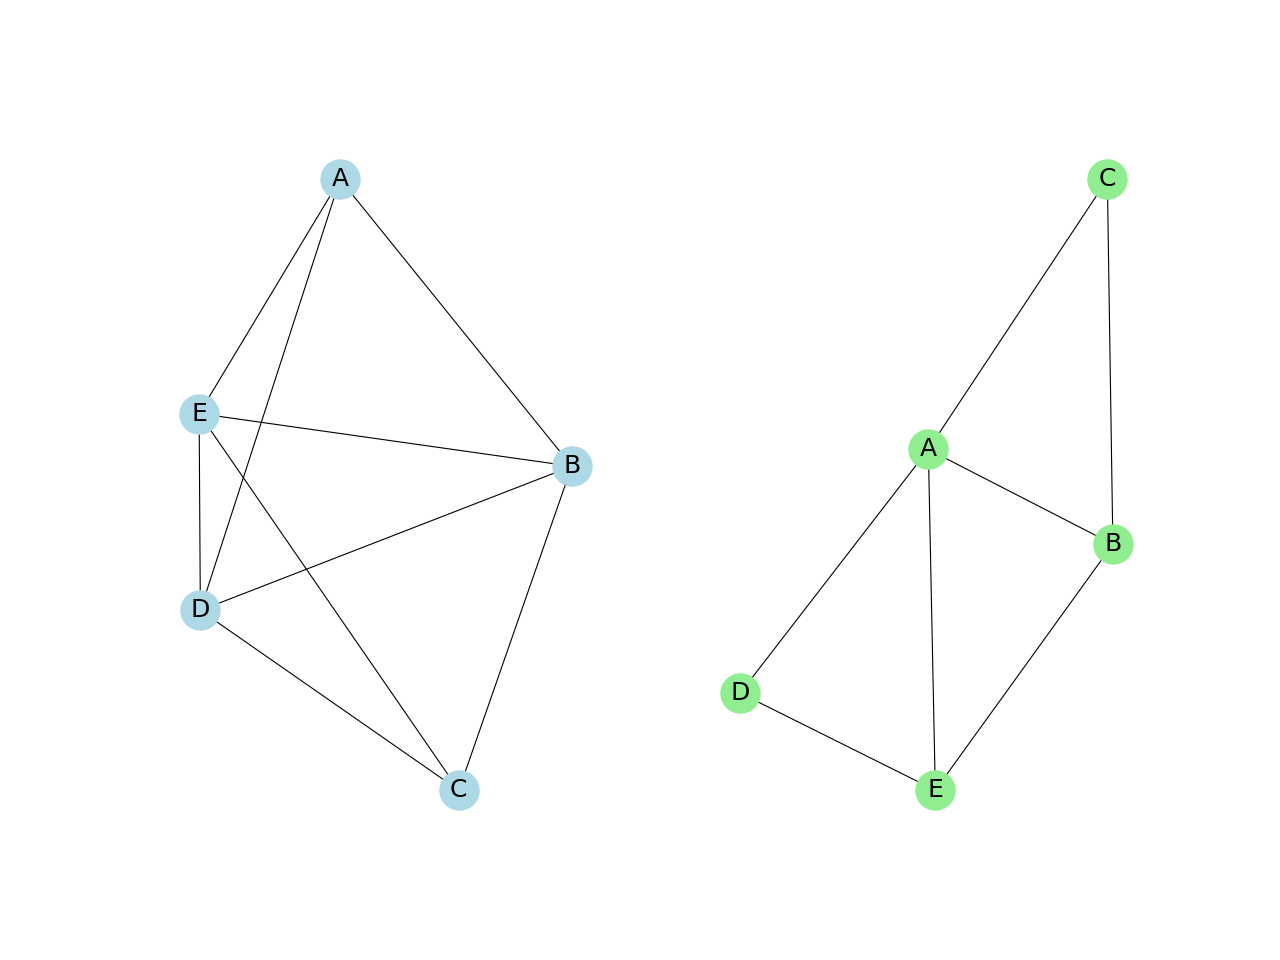
\includegraphics[width=1.0\textwidth]{Graphics/MatrixInNetwork.png}
    \caption{Links ist Netzwerk1 als Graph dargestellt und rechts Netzwerk2}\label{fig:MatrixInNetzwerk}
\end{figure}

Im Grunde können aber für jegliche Netzwerkanalysen beide Varianten verwendet werden. Jedoch werden in dieser Arbeit überwiegend Graphen zur Veranschaulichung und Matrizen für jegliche Berechnungen verwendet, da es leichter ist auf den Datentyp einer Matrix zuzugreifen. Das in Python bereits definierte und verwendete Paket heißt "NetworkX". Dies ist ein Python-Paket für die Erstellung, Bearbeitung und Untersuchung von Struktur, Dynamik und Funktionen komplexer Netzwerke. Dort ist es möglich, einige Features, welche ein Graph aufweist zu veranschaulichen. \\
In dieser Arbeit betrachten wir, wie in \ref{fig:MatrixInNetzwerk} unschwer zu erkenn ist, nur
ungewichtete Netzwerke, um die Zentralitätsmaße, beziehungsweise Netzwerkeigenschaften zu diskutieren.

\section{Einführung in die Grundstruktur von sozialen Netzwerken}
Ein soziales Netzwerk ist eine soziale Struktur, die zwischen Akteuren - Einzelpersonen oder Organisationen - besteht. Es zeigt die Art und Weise, wie Menschen und Organisationen durch verschiedene soziale Vertrautheiten verbunden sind, die von zufälligen Bekanntschaften bis hin zu engen familiären Bindungen reichen. Soziale Netzwerke bestehen aus Knotenpunkten und Verbindungen, deren Wechselwirkung nicht linear ist. Die Person oder Organisation, die am Netzwerk teilnimmt, wird als Knoten bezeichnet. Bindungen sind die verschiedenen Arten von Verbindungen zwischen diesen Knotenpunkten. Bindungen werden nach ihrer Stärke bewertet. Lockere Verbindungen, wie bloße Bekanntschaften, werden als schwache Verbindungen bezeichnet. Starke Verbindungen, wie z. B. Familien oder Cliquen, werden als starke Bindungen bezeichnet. Beispiele für soziale Netzwerke sind unsere Gesellschaft, das Internet, unser Gehirn und zelluläre Interaktionen.
Doch welche grundsätzlichen Eigenschaften muss ein Netzwerk erfüllen, um als $"$soziales Netzwerk$"$ bezeichnet werden zu dürfen? 
Sozialwissenschaftler*innen haben drei Arten von Netzwerken untersucht: egozentrische, soziozentrische und systemoffene
Netzwerke. Egozentrische Netze sind Netze, die mit einem einzigen Knoten oder einer einzigen Person verbunden sind. Um als Netze zu gelten, müssen diese Verbindungen nicht nur Listen von Personen oder Organisationen sein, sondern es müssen auch Informationen über die Verbindungen zwischen diesen Personen oder Organisationen enthalten sein. Im allgemeinen Sprachgebrauch, insbesondere wenn von sozialer Unterstützung die Rede ist, wird jede Liste als Netzwerk betrachtet. Eine Person, die eine große Anzahl guter Freunde hat, auf die sie auf die sie sich verlassen kann, wird ein großes "Netzwerk" genannt. Soziozentrische Netzwerke sind, wie Russell Bernard (persönliche Kommunikation), Netzwerke in einer Box. Netze mit offenen Systemen sind Netze, bei denen die Grenzen nicht unbedingt klar sind, sie liegen nicht in einer Box - zum Beispiel die Elite der Vereinigten Staaten oder die Verbindungen zwischen Unternehmen, oder die Kette der Beeinflusser einer bestimmten Entscheidung oder die Übernahme neuer Praktiken. In gewisser Weise sind dies die interessantesten Netzwerke. Sie sind auch am schwierigsten zu untersuchen. 

Diesen Teil werde ich zu einem anderen Zeitpunkt schreiben müssen weil ich keine Quellen finden, die es gut genug beschreiben was ich genau als Daten brauche.




%*****************************************
%*****************************************
%*****************************************
%*****************************************
%*****************************************
%************************************************
\chapter{Kernfaktoren einer sozialen Netzwerkanalyse}\label{ch:kernfaktoren} % $\mathbb{ZNR}$
%************************************************
In komplexen Netzwerken können einige Knoten als wichtiger angesehen werden als andere. In einem sozialen Netzwerken zeichnen sich wichtige Knoten durch vergleichsweise mehr Verbindungen als andere Knoten aus. Auf das Beispiel \textit{Instagram} bezogen, können solche Knoten Informationen gut verbreiten, sogenannte Influencer. Daher werden diese Knotenpunkte als zentral oder sozial wichtig interpretiert. Die Interpretation der Zentralität ist jedoch nicht eindeutig \cite{GOLBECK201325}. Zum Beispiel im Linienverkehr,
gilt eine Linie als zentral, wenn sie von großen Menschenmengen genutzt und stärker frequentiert wird,
als andere Linien. Die Definition der Zentralität ist also nicht allgemein und hängt von der Anwendung ab. Da es keine allgemeine Definition von Zentralität gibt, wurden mehrere Maße entwickelt, die jeweils spezifische Konzepte berücksichtigen.
Die Zentralität ist deshalb eine Schlüsseleigenschaft komplexer Netzwerke. Sie kann unter anderem das Verhalten dynamischer Prozesse wie beispielsweise eine epidemische Ausbreitung erklären, modellieren und abschätzen, jedoch nicht beschreiben, da es oftmals schwierig ist exakte Aussagen zu tätigen, wenn unbekannte Faktoren in den Datensätzen enthalten sind. \cite{SpringerElbert}. Zudem kann die Zentralität Informationen über die Organisation komplexer Systeme und unsere Gesellschaft liefern. Es gibt viele Metriken zur Quantifizierung der Knotenzentralität in Netzwerken \cite{francisco}.

\section{Zentralitäten}
\label{ch:Zentralitaeten}
Die \textit{Grad-Zentralität} ist die am einfachsten zu berechnende Zentralität. Sie ist definiert durch die Anzahl der \textit{direkten} Verbindungen eines Knoten. Mit der Adjazenzmatrix wird der Grad der Zentralität berechnet, indem die Summe der Elemente der betroffenen Zeile $i$ berechnet wird.
Mathematisch formuliert, wird folgende Formel verwendet: 
\begin{equation}
     k_i &= \sum_{j=1}^{N} A_i_j 
     \label{degree}
\end{equation}

Wobei $A$ die Adjazenzmatrix beschreibt, $N$ die Anzahl an Knoten darstellt und $i$, $j$ die Knoten. \\
Da es sich bei der \textit{Grad-Zentralität} um die einfachste Zentralität handelt, wird meist davon ausgegangen, dass Knoten mit vielen Verbindungen, daher mit einer hohen Zentralität, sich visuell betrachtet im Zentrum eines Netzwerkers befinden. Dies hat jedoch einige Nachteile, denn Knoten mit der höchsten \textit{Grad-Zentralität} können sich auch visuell am Rand des Netzes befinden, was dazu führt, dass die \textit{Grad-Zentralität} nicht als lokales Maß betrachtet wird. Zudem sollte hervorgehoben werden, dass bei der \textit{Grad-Zentralität} nur ein- beziehungsweise ausgehende Kanten gezählt werden. Dies sagt zwar aus, dass ein solcher Knoten, auf das soziale Netzwerk bezogen, eine beliebte oder sehr bekannte Person ist, doch es ist dadurch keine Aussage über die Macht oder den Einfluss der Person möglich. Als extremes Beispiel, warum die \textit{Grad-Zentralität} nicht immer optimal zur Netzwerkanalyse ist, diene ein Netzwerk mit einer großen, dichten Gruppen von Knoten. Als dichte Gruppe ist hierbei eine Ansammlung von Knoten zu verstehen, welche sich alle nah beieinander befinden. Diese machen den größten Teil des Graphen aus, welcher auch als Kern des Netzes bezeichnet wird. Jedoch kann (visuell betrachtet) weit außerhalb des Kerns, entlang einer Kette von Knoten mit niedrigem Grad, ein Knoten liegen, welcher mit einer großen Anzahl von Knoten verbunden ist. Ein solcher Knoten hätte einen hohen Grad an Zentralität, obwohl er weit vom Kern des Netzes und den meisten Knoten entfernt ist \cite{SpringerElbert}. 
Um solche Faktoren mit berücksichtigen zu können, wird ein weiterer Faktor in die Berechnung integriert, nämlich die Weglänge. \\

Diese spielt eine wichtige Rolle bei der \textit{Nähe-Zentralität}, 
denn die Knotenzentralität kann auch anhand der kürzesten Wege definiert werden. Der Abstand zwischen zwei Knoten $i$ und $j$ ist gegeben durch die Anzahl der Kanten, welche sie möglichst direkt verbindet. Ein zentraler und daher wichtiger Knoten liegt, bezogen auf den Abstand, nahe an allen anderen Knoten des Netzes. Dieser Gedanke ist im Maß der sogenannten \textit{Nähe-Zentralität} oder \textit{Closeness-Centrality} enthalten. Diese wird durch den durchschnittlichen Abstand eines jeden Knotens zu allen anderen Knoten definiert. Mathematisch wird die Formel wie folgt beschrieben: 

\begin{equation}
     C_i &= \frac{N}{\sum_{j=1, j \not{=}i}^{N} d_i_j }
\end{equation}

Dabei ist mit $d_i_j$ der kürzeste Weg zwischen $i$ und $j$ gemeint und mit $N$ erneut die Anzahl an Knoten im Netzwerk \cite{SpringerElbert}. Die \textit{Nähe-Zentralität} ist vor allem dann sehr geeignet, wenn Prozesse über kurze Wege charakterisiert werden sollen. Beispielsweise kann der hierarchischen Aufbau eines Unternehmens in einem sternförmigen Graphen dargestellt werden. In der Mitte des Graphen befindet sich der Vorstand, der in engem Kontakt mit den jeweiligen Abteilungsleitern steht. Die Abteilungsleiter sind, neben dem Vorstand, wiederum in sehr nahem Kontakt mit ihren jeweiligen Mitarbeitern ihrer Abteilung. Wenn nun ausschließlich anhand der \textit{Grad-Zentralität} argumentiert wird, sind die Abteilungsleiter die wichtigsten Knoten im Graphen. Jedoch haben diese nicht die niedrigste \textit{Nähe-Zentralität}, denn der Vorstand hat, da sich dieser Knoten visuell in der Mitte des Graphen befindet, zu allen anderen Knoten entweder einen oder zwei Kanten Abstand. Die einzelnen Abteilungsleiter haben aber, im worst-case Fall, zu anderen Angestellten aus anderen Abteilungen zwei bis drei Kanten Abstand. Dementsprechend ist es nicht ausreichend nur eine Zentralität bei der Analyse von \textit{sozialen Netzwerken} zu betrachten. Bei der \textit{Nähe-Zentralität} weisen die meisten komplexen Netze eine geringe durchschnittliche Länge des kürzesten Weges auf. Dies ist damit zu begründen, dass die durchschnittliche Entfernung mit dem Logarithmus über die Anzahl der Knoten zunimmt. 
Daher liegt das Verhältnis zwischen dem größten und dem kleinsten Abstand
in der Größenordnung $log(N)$, da der minimale Abstand gleich eins ist. In den meisten real existierenden
Netzwerken beträgt dieses Verhältnis etwa 6 oder weniger. Es kann also mehrere Knoten mit der gleichen
Zentralität geben, obwohl sie bei der Informationsverbreitung unterschiedliche Rollen spielen können. Daher ist die \textit{Nähe-Zentralität} besser geeignet für räumliche Netze, bei denen die Abstände zwischen den Knoten größer sind als in zufälligen Netzen mit der gleichen Anzahl von
Knoten und Verbindungen \cite{SpringerElbert}.\\

Die \textit{Betweenness-} oder \textit{Zwischen-Zentralität} hingegen misst, wie wichtig ein Knoten für die kürzesten Pfade durch das Netz ist. Um diese Zentralität für einen Knoten $N$ zu berechnen, wird in dieser Methode eine Gruppe von Knoten ausgewählt und alle kürzesten Wege zwischen diesen Knoten gesucht. Dann wird der Anteil dieser kürzesten Wege berechnet, die den Knoten $N$ einschließen. Wenn es beispielsweise 7 kürzeste Wege zwischen einem Knotenpaar gibt und 5 davon durch den Knoten N führen, dann wäre der Anteil $5/7=0.714$. Dieser Vorgang wird für jedes Knotenpaar im Netz wiederholt. Anschließend werden die berechneten Brüche addiert, wodurch die \textit{Zwischen-Zentralität} des Knotens $N$ generiert wird. Mathematisch formuliert sieht die Formel dann wie folgt aus: 
\begin{equation}
     B_i &= \sum_{(a-b)}\frac{\eta(a,i,b)}{\eta(a,b)}
\end{equation}
Hierbei bezeichnet $\eta(a,i,b)$ die Anzahl der kürzesten Wege zwischen den Knoten $a$ und $b$ die durch den Knoten $i$ führen. Zudem stellt $\eta(a,b)$ die Gesamtzahl der kürzesten Wege zwischen $a$ und $b$ dar. 
Diese Zentralität, basierend auf dem \textit{random walk-Algorithmus} und ist gegeben durch die erwartete Anzahl der Besuche von jedem Knoten $i$ während einer zufälligen Schrittfolge durch den Graphen:
\begin{equation}
     B_i &= \sum_{a=b}^{N}\sum_{b=1}^{N}w(a,i,b)
\end{equation}
dabei ist $w(a,i,b)$, wie oben bereits beschrieben für $\eta(a,i,b)$, die Anzahl der kürzesten Wege zwischen den Knoten $a$ und $b$, die durch den Knoten $i$ führen. Die Lösung wird daher nur angenähert.
Die \textit{Zwischen-Zentralität} ist eines der am häufigsten verwendeten Zentralitätsmaße. Sie gibt an, wie wichtig ein Knoten für den Informationsfluss von einem Knoten des Netzes zu einem anderen ist. In gerichteten Netzwerken kann die \textit{Zwischen-Zentralität} mehrere Bedeutungen haben \cite{SpringerElbert}. Einem Nutzer $Anton$ mit hoher \textit{Zwischen-Zentralität} folgen möglicherweise viele andere Nutzern, welche jedoch nicht denselben Personen folgen wie der Nutzer $Anton$ selbst. Dies würde darauf hindeuten, dass der Nutzer $Anton$ viele Anhänger oder Follower hat. Es kann aber auch sein, dass der Nutzer $Anton$ weniger Follower hat, diese aber dafür mit vielen Knoten verbindet, die ansonsten weit entfernt sind. Daher ist es enorm wichtig die Richtung der Kanten eines Knotens zu kennen, um die Bedeutung der Zentralität zu verstehen. \\

Die \textit{Eigenvektor-}oder \textit{Eigenwert-Zentralität} misst die Bedeutung eines Knotens, wobei die Bedeutung seiner Nachbarn berücksichtigt wird. Deshalb wird sie manchmal verwendet, um den Einfluss eines Knotens im Netzwerk zu messen. Sie wird durch eine Matrixberechnung ermittelt, um den so genannten \textit{Haupteigenvektor} anhand der Adjazenzmatrix zu bestimmen. Mathematisch betrachtet ist die \textit{Eigenvektor-Zentralität} die komplizierteste, der in dieser Arbeit betrachteten Zentralitäten.\\
Wird nun die Tatsache betrachtet, dass ein Akteur zentraler ist, wenn er in Beziehung zu weiteren Akteuren steht, die selbst zentral sind, so kann argumentiert werden, dass die Zentralität eines Knotens nicht nur von der der Anzahl seiner Nachbarknoten abhängt, sondern auch von deren Zentralitätswert. Beispielsweise definiert Bonacich (1972) die Zentralität $c(v_i)$ eines Knotens $v_i$ als positives Vielfaches der Summe der benachbarten Zentralitäten. Als Formel mathematisch dargestellt sieht dies folgendermaßen aus:
\begin{equation}
     \lambda c(v_i) = \frac{1}{\lambda} \sum_{j=1}^{N}a_{ij}c(v_j) \forall i
\end{equation} oder umformuliert:  
\begin{equation}
     c(v_i) = \sum_{j=1}^{N}a_{ij}c(v_j) \forall i
\end{equation}
Hierbei repräsentiert $a_{i,j}$ die Werte der Adjazenzmatrix $A$ und $\lambda$ einen konstanten Faktor. \\
In Matrixschreibweise mit $c = (c(v_1), ...., c(v_n))$ bedeutet dies auch:
\begin{equation}
     Ac = \lambda c
\end{equation}
Diese Art von Gleichung wird durch die Eigenwerte und Eigenvektoren von $A$ gelöst.
Aus der gesamten Menge an verschiedenen Eigenvektoren, soll es nur eine geeignete Lösung geben. 
Dieser Eigenvektor kann dann direkt als Zentralitätsmaß dienen. Da $A$ die Adjazenzmatrix eines ungerichteten (zusammenhängenden) Graphen ist, ist $A$ nicht negativ und aufgrund des Satzes von Perron-Frobenius, existiert ein Eigenvektor des maximalen Eigenwerts mit ausschließlich nicht negativen, also positiven, Einträgen \cite{brittaRuhnau}.

\section{Cliquen und Brücken}
\label{ch:CliquenBrücken}
Eine Clique ist laut Definition ein Teilgraph, aus mindestens drei Knoten bestehend, die zudem alle benachbart zueinander sind. Streng bezeichnet handelt es sich bei einer Clique um eine zusammenhängende Untergruppe. Eine Clique kann ebenso als Ansammlung von Akteuren gesehen werden, die sich gegenseitig wählen, jedoch wählt kein anderer Akteur dieser Gruppe weitere Akteure aus weiteren Gruppen und wird auch nicht von anderen Akteuren gewählt. Es ist zu beachten, dass sich Cliquen in einem Graphen auch überlappen können, also derselbe Satz von Knoten zu mehr als nur einer Clique gehören kann. Zu beachten ist, dass eine vollständige Clique nicht in einer anderen Clique enthalten sein kann, denn sonst wäre die kleinere Clique nicht mehr maximal. Die Cliquendefinition ist vor allem nützlich, für die Untersuchung der Eigenschaften einer Untergruppe beziehungsweise eines Subgraphen \cite{wasserman1994social}. Was genau damit gemeint ist, ist in folgendem Plot zu sehen: 
\FloatBarrier
\begin{figure}[htb!]
    \centering
    %\hspace*{-1cm}
    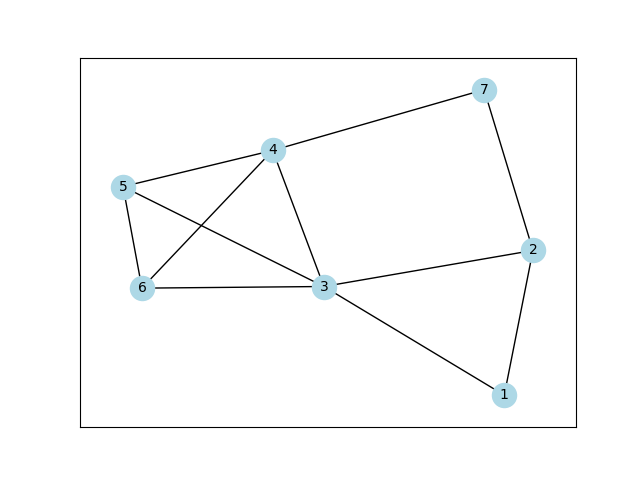
\includegraphics[width=0.55\textwidth]{Graphics/Clique.png}
    \caption{Graph mit den Cliquen (1, 2, 3) und (3, 4, 5, 6)}
    \label{fig:Clique}
\end{figure}

\newpage
Wichtig ist hierbei, dass es sich bei (2, 3, 4, 7) um keine Clique handelt, da keine Verbindung zwischen den Knoten \textbf{4 und 2} und ebenso keine Verbindung zwischen den Knoten \textbf{3 und 7} besteht.
Neben den Cliquen sind auch Brücken eine wichtige Diskussions- und Analysierungsgrundlage für Graphen beziehungsweise in unserem Fall für \textit{soziale Netzwerke}. Wenn von Brücken (bzw. englisch Bridge) die Rede ist, sind Verbindungen zwischen zwei Knoten gemeint. Jedoch handelt es sich um die einzige Verbindung zwischen diesen Knoten und deren Kontakten \cite{bridge}. Ein Beispiel für Brücken im Graphen liefert folgender Plot:

\FloatBarrier
\begin{figure}[htb!]
    \centering
    %\hspace*{-1cm}
    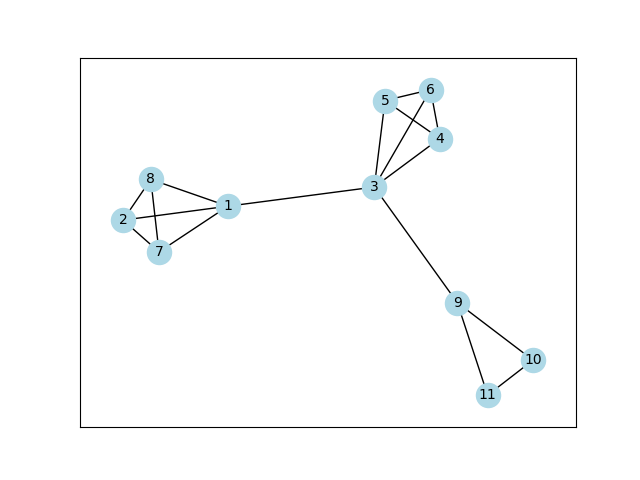
\includegraphics[width=0.55\textwidth]{Graphics/Bridge.png}
    \caption{Graph mit den Brücken (1, 3) und (3, 9)}
    \label{fig:Bridge}
\end{figure}
Hierbei ist gut zu erkennen, dass die drei Subgraphen durch \textit{Brücken} miteinander verbunden sind. Neben den Brücken sind in Abbildung \ref{fig:Bridge} die Cliquen (1,2,7,8), (3,4,6,5) und (9,10,11) enthalten. Zu beachten ist, dass es sich bei beispielsweise (1,7,8) oder (4,5,6) um keine Cliquen handelt. Wenn nun diese Brücken und Cliquen im Zusammenhang mit den Zentralitäten betrachtet werden und die oben aufgeführten Formeln der Zentralitäten auf den Graphen \ref{fig:Bridge} angewendet werden, erhält man die unten stehende Tabelle \ref{table:TableCliqueBridg}. Eine Berechnung für Abbildung \ref{fig:Clique} ist nicht nötig, da in Abbildung \ref{fig:Bridge} ebenfalls Cliquen und zusätzlich Brücken enthalten sind:
\begin{table}[h!]
\centering
\footnotesize
\caption{Werte Abbildung \ref{fig:Bridge}}
\label{table:TableCliqueBridg}
\begin{tabular}{lccccc}\toprule
\textbf{Node} & \textbf{Grad-Zentr.} &\textbf{Nähe-Zentr.} &\textbf{Betweeness-Zentr.} & \textbf{Eigen.-Zentr.} \\
 &\\\midrule
  3 & 0.5 & 0.666667 & 0.733333 & 0.470733  \\
  1 & 0.4 & 0.555556 & 0.466667 & 0.387253  \\
  4 & 0.3 & 0.454545 & 0        & 0.340195  \\
  6 & 0.3 & 0.454545 & 0        & 0.340195  \\
  5 & 0.3 & 0.454545 & 0        & 0.340195  \\
  2 & 0.3 & 0.4      & 0        & 0.279871  \\
  7 & 0.3 & 0.4      & 0        & 0.279871  \\
  8 & 0.3 & 0.4      & 0        & 0.279871  \\
  9 & 0.3 & 0.5      & 0.355556 & 0.184986  \\
 10 & 0.2 & 0.357143 & 0        & 0.0776041 \\
 11 & 0.2 & 0.357143 & 0        & 0.0776041 \\
       
  \\\bottomrule
 \end{tabular}
 \end{table}

Direkt fällt auf, dass die Werte spaltenweise sehr ähnlich zueinander sind. Bei der \textit{Gradzentralität} sind die Knoten \textbf{3} und \textbf{1} mit einem Wert von \textbf{0.5} und \textbf{0.4} am höchsten. Interessant, denn dabei handelt es sich um die Knoten, die unsere \textit{Brücke} bilden. Bei den Knoten \textbf{3} und \textbf{1} fällt des weiteren auf, dass diese Knoten bei der \textit{Nähe-}, \textit{Zwischen-} und \textit{Eigenvektor-Zentralität} ebenfalls am höchsten sind. Das heißt, die Vermutung liegt nahe, dass die Knoten eines Graphen, die Cliquen bilden, relativ ähnliche \textit{Zentralitätswerte} aufweisen beziehungsweise die Varianzen geringer sind. Aber vor allem erwähnenswert ist, dass in der Tabelle \ref{table:TableCliqueBridg} lediglich bei den Knoten, welche die \textit{Brücke} bilden, Werte ungleich \textit{Null} in der Spalte \textit{Betweeness-Zentr.} auffindbar sind. Dies sollte für den weiteren Teil der Arbeit in Erinnerung bleiben. 


\section{Soziale Netzwerk-Eigenschaften}
\label{ch:eigenschaftenTabelle}
Die wichtigsten Eigenschaften eines sozialen Netzwerks sind die folgenden: 
\begin{table}[h!]
\footnotesize
\caption{Eigenschaften eines sozialen Netzwerks}
\label{TableEigenschaften}
%\centering
\begin{tabular}{lcc}\toprule 
\textbf{Eigenschaft} &\textbf{Beschreibung} \\
 &\\\midrule
 \\
  \textbf{Cluster} & Ein soziales Netzwerk sollte aus mehreren Cluster oder Subgraphen \\ &bestehen. Diese können in ihrer Größe und Anzahl stark variieren   \\
  \\
  \textbf{Brücke} & Die einzelnen Cluster sind über Brücken miteinander verbunden \\
  \\
  \textbf{Clique} & In den Cluster sollten Cliquen vorzufinden sein, d.h mindestens \\
  & drei Knoten existieren die untereinander alle miteinander verbunden sind \\
  \\
  \textbf{Grad-Zentralität} &  Die einzelnen Knoten der Cluster sollten unterschiedliche Grad-\\
  & Zentralitäten haben. Hohe Zentralitäten bedeuten, dass es sich \\
  & um wichtige Knoten handelt, niedrige Werte, dass es weniger \\ 
  & wichtige Knoten sind. Wichtig ist jedoch, dass es nicht aus-\\
  & schließlich wichtige oder ausschließlich unwichtige Knoten gibt.  \\
  \\
  \textbf{Nähe-Zentralität} & Auch hier sollen die Knoten im Cluster unterschiedliche Wert \\
  & aufweisen. Hohe Werte bedeuten, die Knoten sind nah bei- \\
  & einander, haben kurze Wege zueinander. Niedrige Werte \\
  & bedeuten, dass die Knoten weite Entfernungen zueinander haben.\\
  \\
  \textbf{Zwichen-Zentralität} & Hier wird die Wichtigkeit der Nachbar-Knoten in Relation \\
  & bewertet. Hohe Werte bedeuten, dass diese Knoten oft \\
  &für den kürzesten Weg verwendet werden. Niedrige Werte, \\
  & dass diese Knoten nicht für die kürzesten Wege relevant sind.\\
  
  \\\bottomrule
 \end{tabular}
 \end{table}
Natürlich gibt es deutlich mehr Faktoren als die in Tabelle \ref{TableEigenschaften} dargestellten. Jedoch sind diese die primären Eigenschaften, welche in dieser Arbeit berücksichtigt werden.
Nun sind die wichtigsten Eigenschaften der, in dieser Arbeit betrachteten und verwendeten, Metriken wie Clique, Größe oder Brücken bekannt und eingeführt. Manche Zentralitäten wurden oberflächlicher erklärt als andere, weil sie weniger relevant für die Untersuchung der sozialen Netzwerke sind. In Zukunft wird in dieser Arbeit bei \textit{typischen Eigenschaften} von Netzwerken stets auf Tabelle \ref{ch:eigenschaftenTabelle} verwiesen.

\newpage
\section{Ein typisches soziales Netzwerk}
Nachdem nun alle Zentralitäten, deren Berechnungen und weitere wichtige Eigenschaften von sozialen Netzwerken bekannt sind, ist es an der Zeit ein Musterbeispiel für ein soziales Netzwerk zu betrachten. Das bekannteste Netzwerk ist natürlich Facebook. Bei dieser sozialen Plattform ist die geeignetste Darstellung ein \textit{ungerichteter} Graph. Bei Instagram hingegen, ein \textit{gerichtet} Graph. Denn hier gibt es neben Leuten, denen wir folgen, die eigenen Follower \cite{fbInsta}. Die Knoten sind sogenannte \textit{Nutzer} und die \textit{Kanten} sind Verbindungen zwischen ihnen. Zu beachten ist, dass sowohl \textit{Knoten} als auch \textit{Kanten} Attribute zugewiesen werden können. Knotenattribute in Facebook können zum Beispiel \textit{Geschlecht}, \textit{Ort}, \textit{Alter} usw. sein, und Kantenattribute können \textit{Datum der letzten Unterhaltung zwischen zwei Knoten}, \textit{Anzahl der Likes}, \textit{Datum der Verbindung} usw. sein \cite{GOT}.
Im folgenden wird ein, auf den ersten Blick und nach den Eigenschaften von \\ 
Tabelle \ref{ch:eigenschaftenTabelle} typisch erscheinendes, soziales Netzwerk betrachtet. Es muss jedoch stets klar sein, dass es sich hierbei um den Datensatz eines fiktiven Fantasy Drama handelt \cite{GOT} und es daher zu Unstimmigkeiten bei den Ergebnissen und der Analyse kommen kann.

\FloatBarrier
\begin{figure}[h!]
    \centering
    %\hspace*{-1cm}
    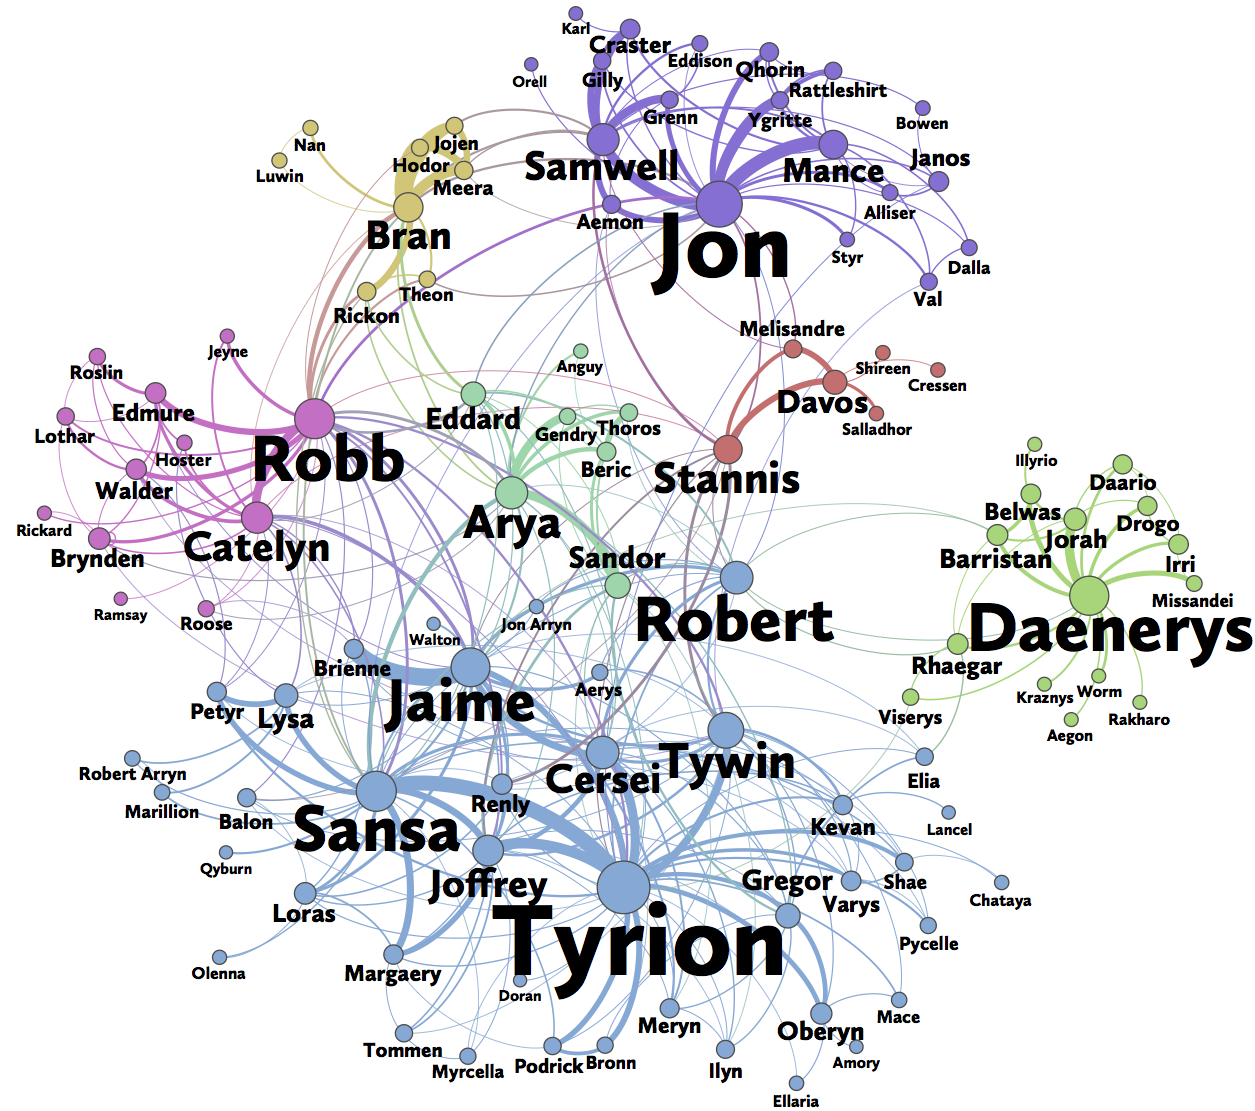
\includegraphics[width=0.75\textwidth]{Graphics/got-network.png}
    \caption{Game of Thrones social Network,\\
    Quelle: https://predictivehacks.com/social-network-analysis-of-game-of-thrones/,\\ Stand: 28.03.2022}
    \label{fig:GameOfThrones}
\end{figure}

Das Netzwerk besteht aus $796$ Knoten und $2823$ Kanten. Insgesamt daher aus $796$ Charakteren aus \textit{Game of Thrones (GOT)}.
In dieser \textit{sozialen Netzwerk Analyse} tauchen auch bisher unbekannte Messungen auf, die aber im Interpretations-Teil dieser Arbeit ebenfalls aufgegriffen werden. Beispielsweise beträgt der \textit{Durchmesser} des GOT Graphen $9$. Das heißt, wenn die kürzeste Pfadlänge von jedem Knoten zu allen anderen Knoten berechnet ist, ist der Durchmesser die längste aller berechneten Pfadlängen. Die durchschnittlich kürzeste Pfadlänge beträgt $3.41$. Diese wird aber zu einem späteren Zeitpunkt analysiert. In Abbildung \ref{fig:GameOfThrones} ist gut zu erkennen, welche Knoten eine zentrale Rolle in diesem spielen. Hierfür wird mit der Knoten-Größe in der Abbildung \ref{fig:GameOfThrones} variiert. Große Knoten implizieren, dass es sich um einen wichtigen Knoten in dem Teilgraphen handelt und kleine, dass es sich um weniger relevante Knoten handelt \cite{GOT}. 
\begin{table}[h!]
\footnotesize
\caption{Werte GOT Graph}
\label{TableGOT}
\begin{tabular}{lccccc}\toprule 
\textbf{Charakter} &\textbf{Grad-Zentr.} & \textbf{Charakter} &\textbf{Nähe-Zentr.}  & \textbf{Charakter} &\textbf{Betweeness-Zentr.} \\
 &\\\midrule
  Tyrion Lannister & 0.1535  & Tyrion Lannister & 0.4763 & Jon Snow& 0.1921   \\
  Jon Snow & 0.1434 & Robert Baratheon & 0.4593 & Tyrion Lannister & 0.1622   \\
  Jaime Lannister & 0.1270  & Eddard Stark& 0.4558& Daenerys Targaryen & 0.1184   \\
  Cersei Lannister & 0.1220 & Cersei Lannister & 0.4545 & Theon Greyjoy & 0.1113   \\
  Stannis Baratheon & 0.1119 & Jaime Lannister & 0.4520 & Stannis Baratheon & 0.1101   \\
       
  \\\bottomrule
 \end{tabular}
 \end{table}
Wenn diese Knoten in der Abbildung \ref{fig:GameOfThrones} gesucht werden, ist visuell direkt ersichtlich, dass es sich hierbei um die Knoten mit den meisten Verbindungen handelt. Oftmals ist leider bei den abgebildeten Graphen nicht eindeutig erkennbar, ob es sich hierbei um Kanten handelt, welche zwei Knoten direkt miteinander verbinden, oder die Kanten lediglich am Knoten vorbei verlaufen. Deshalb ist es wichtig, die Werte aus der Tabelle \ref{TableGOT} zu analysieren. Hier fällt bei den Spalten \textit{Charakter} auf, dass \textit{Tyrion -Lannister} in allen aufgeführt wird. Das heißt, dass dieser Knoten im Graphen (visuell betrachtet) sowohl zentral liegen, und zudem kurze Abstände zu den anderen Knoten nachweisen muss. Zudem müssen über diesen Knoten die häufigsten kürzesten Wege verlaufen. Bei der Abbildung \ref{fig:GameOfThrones} fällt ebenfalls auf, dass der Knoten, beziehungsweise Charakter, $Tyrion$  heraus sticht. Er ist von den meisten Knoten und Kanten umgeben. Da drei der fünf wichtigsten Knoten in der Spalte $Grad-Zentr.$ den gleichen zweiten Namen tragen, liegt die Vermutung nahe, dass es sich hier um Knoten handelt, die auch visuell betrachtet sehr nah beieinander liegen müssem. Beim Betrachten des Graphen bestätigt sich diese Vermutung direkt, denn alle drei Knoten befinden sich im blauen Teilgraphen. Zudem handelt es sich bei dem Namen $"Lannister"$ um ein Adelshaus in der US-amerikanischen Fantasy-Fernsehserie \textit{Game of Thrones} was die starke Verbindung und Nähe zueinander begründet. Außerdem fällt sofort auf, dass drei der fünf Charaktere in der Spalte \textit{Nähe-Zentr.} die selben sind, wie die wichtigsten Charaktere bezüglich der \textit{Grad-Zentr.} Wieder bedeutet das, dass diese Charaktere sowohl zentral im Graphen liegen müssen als auch die kürzesten Wege zu anderen Knoten besitzen. Die Betrachtung von Abbildung \ref{fig:GameOfThrones} bestätigt dies sofort. Zudem weist der Graph auch einige Cliquen auf. Die relevanteste und vor allem größte Clique befindet sich im blauen, grünen, ein Knoten im roten und zwei Knoten im pinken Teilgraphen. Aus dem Kapitel über Brücken und Cliquen \ref{ch:CliquenBrücken} ist bekannt, dass die Knoten mit den höchsten Zentralitäten höchstwahrscheinlich eine Clique darstellen und es sich vor allem bei den Knoten mit hohen \textit{Zwischen-Zentralität} um Brücken handelt. Jedoch wird die Analyse dieses sozialen Netzwerks nicht weitergeführt, sondern auf die Analyse des selbst generierten sozialen Netzwerks fokussiert. Auch auf die Frage, welcher mathematischen bzw. stochastischen Verteilung die Zentralitäten entsprechen und warum eine solche Untersuchung sinnvoll ist, wird zu einem späteren Zeitpunkt eine Antwort gegeben.

%*****************************************
%*****************************************
%*****************************************
%*****************************************
%*****************************************

%----------------------------------------------------------------------------------------
%	PART 2
%----------------------------------------------------------------------------------------
\cleardoublepage
\ctparttext{Nun folgt der Teil der Arbeit, in dem selbst generierte soziale Netzwerke untersucht werden. Handelt es sich bei den generierten Netzwerken tatsächlich um soziale Netzwerke und erfüllen sie alle Ansprüche bezüglich der Zentralitäten und sonstigen Eigenschaften von sozialen Netzwerken? Dies sind einige Fragen, die in diesem zweiten Teil der Arbeit beantwortet werden sollen.}
\part{Der praktische Teil}\label{pt:prakticalPart}

%----------------------------------------------------------------------------------------
%	Chapters
%*****************************************
\chapter{Der Graphen Generator}\label{ch:generierung}
%*****************************************
Nun beschäftigt sich diese Arbeit im weiteren damit, wie typische soziale Netzwerke generiert werden können. 
Zunächst bietet es sich an dieser Stelle oftmals an, da Facebook und Instagram der Informationspflicht unterliegen, seine eigenen social Media Daten anzufordern. Meist spiegelt dieser Datensatz gelikete und kommentierte Posts der Nutzer*innen wieder, oder verfasste Nachrichten und gesuchte Inhalte.
Bei den ersten Visualisierungsversuchen wird bereits klar, dass diese Daten für eine wissenschaftliche Arbeit nicht brauchbar sind, da es sich bei den erstellten Plots und Ergebnissen nicht um \textit{ typische soziale Netzwerke} aus Tabelle \ref{TableEigenschaften} handelt. Vielmehr bestehen diese meist aus einem Kernknoten, also einem sogenannten sternförmigen Graphen. Plots wie Abbildung \ref{fig:OwnData} sind bei der Visualisierung der eigenen Daten entstanden. Diese besteht aus unzähligen einzelnen Teilgraphen, welche lediglich eine weitere Verbindung aufweisen. Auch sind keine Cliquen oder Brücken in solchen Graphen zu finden, was ebenfalls dafür spricht, dass es sich um kein \textit{typisches soziales Netzwerk} handelt. \\
\FloatBarrier
\begin{figure}[h!]
    \centering
    %\hspace*{-1cm}
    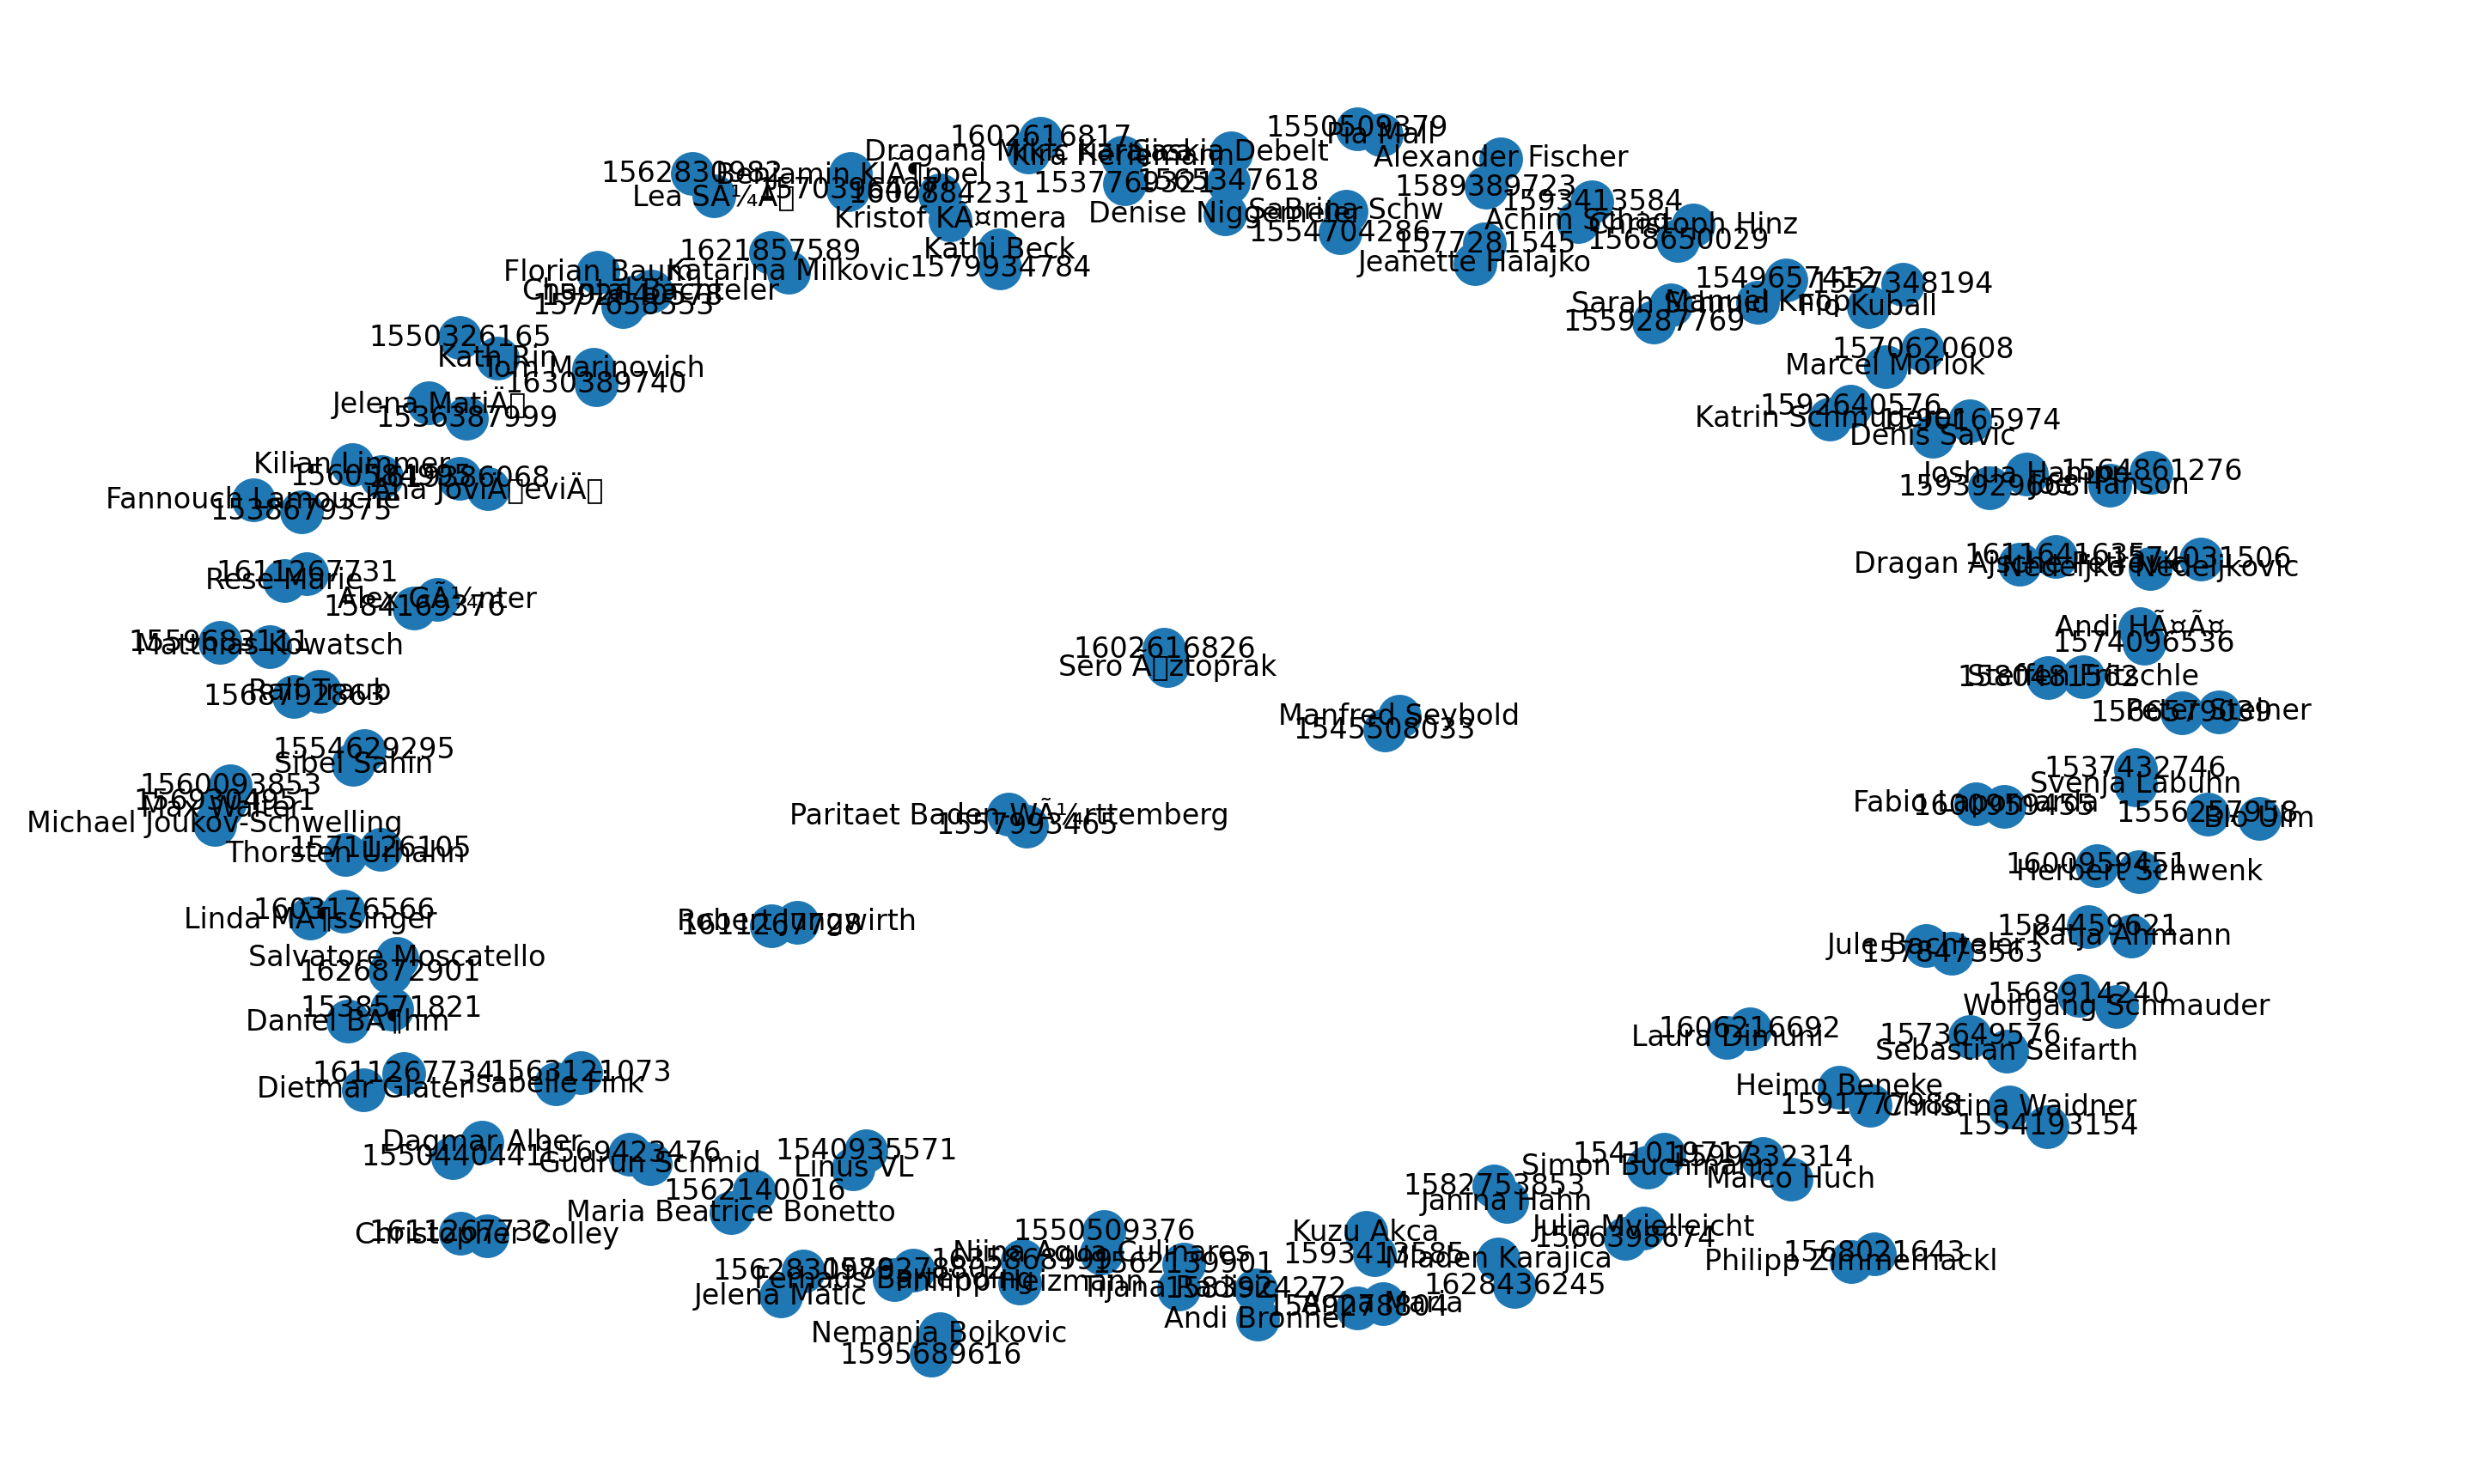
\includegraphics[width=0.7\textwidth]{Graphics/PlotOwnData.png}
    \caption{Erste Versuche eines Sozialen Netzwerks, \\
    selbst erstellt}
    \label{fig:OwnData}
\end{figure}
\FloatBarrier

Eine weitere Schwierigkeit ist bei diesen Graphen die Interpretation der Kanten, denn diese ist teilweise nicht eindeutig. 
Facebook gibt lediglich IDs bekannt, doch welche Bedeutung diese haben ist unbekannt aber im Endeffekt auch nicht relevant für diese Arbeit.

\section{Generierung eines sozialen Netzwerks} 
Bei einer endlichen Anzahl von Knoten \textit{n} gibt es auch eine endliche Anzahl von möglichen Graphen, die aus diesen Knoten erzeugt werden können. Hierbei wächst die Anzahl der Graphen mit \textit{n} Knoten exponentiell.
Ein Zufallsgraph ist nur einer dieser Graphen, der durch einen Zufallsprozess erzeugt werden kann.
Wenn von \textit{Zufallsgraphen} die Rede ist, wird in den meisten Fällen das \textit{Erdős-Rényi-Modell} als Graphengenerator verwendet (benannt nach den Mathematikern Paul Erdős und Alfréd Rényi). Ein wichtiges Kriterium von, auf diese Weise erzeugten Zufallsgraphen ist, dass alle Konstellationsmöglichkeiten des Graphen gleichverteilt erzeugt werden \cite{Generators}.
Neben dem Erdős-Rényi-Modell, gibt es noch viele weitere Methoden zur zufälligen Netzwerkmodellierung \cite{Generators}.
\begin{itemize}
    \item Die \textit{dense$\_$gnm$\_$random$\_$grap-Modellierung} liefert einen Zufallsgraphen.
    Bei dem Modell wird ein Graph gleichmäßig zufällig aus der Menge aller Graphen mit einer gegebenen Anzahl an Knoten und Kanten ausgewählt.
    \item Bei der \textit{Newman–Watts–Strogatz small-world graph-Modellierung} wird zunächst ein Ring mit $n$ Knoten erzeugt. Dann wird jeder Knoten im Ring mit seinen $k$ nächsten Nachbarn verbunden (oder $k - 1$ Nachbarn, wenn $k$ ungerade ist). Anschließend wird für jede Kante im Ring mit $k$ nächsten Nachbarn, mit der Wahrscheinlichkeit $p$, eine neue Kante hinzugefügt.
    \item Die \textit{random$\_$regular$\_$graph-Modellierung} gibt einen zufälligen regulären Graphen mit $n$ Knoten zurück. Das heißt, alle Knoten besitzen gleich viele Nachbarn als somit den selben Grad.
    Der resultierende Graph hat keine Selbstschleifen oder parallele Kanten.
    \item Die \textit{barabasi$\_$albert$\_$graph-Modellierung} hingegen liefert einen Zufallsgraphen nach dem Barabási-Albert-Präferenzmodell.
    Ein Graph mit $n$ Knoten wird durch Anhängen neuer Knoten mit jeweils $m$ Kanten erzeugt, die bevorzugt an bestehende Knoten mit hohem Grad angehängt werden.
    \item Die \textit{powerlaw$\_$cluster$\_$graph-Modellierung} ist im Wesentlichen das\\ Barabási-Albert-Wachstumsmodell mit dem zusätzlichen Schritt, dass für jede zufällige Kante die Chance besteht, dass ebenfalls eine Kante zu einem seiner Nachbarn besteht (und damit ein Dreieck entsteht) \cite{Generators}.
\end{itemize}

\FloatBarrier
\begin{figure}[h!]
    \centering
    \hspace*{-1.5cm}
    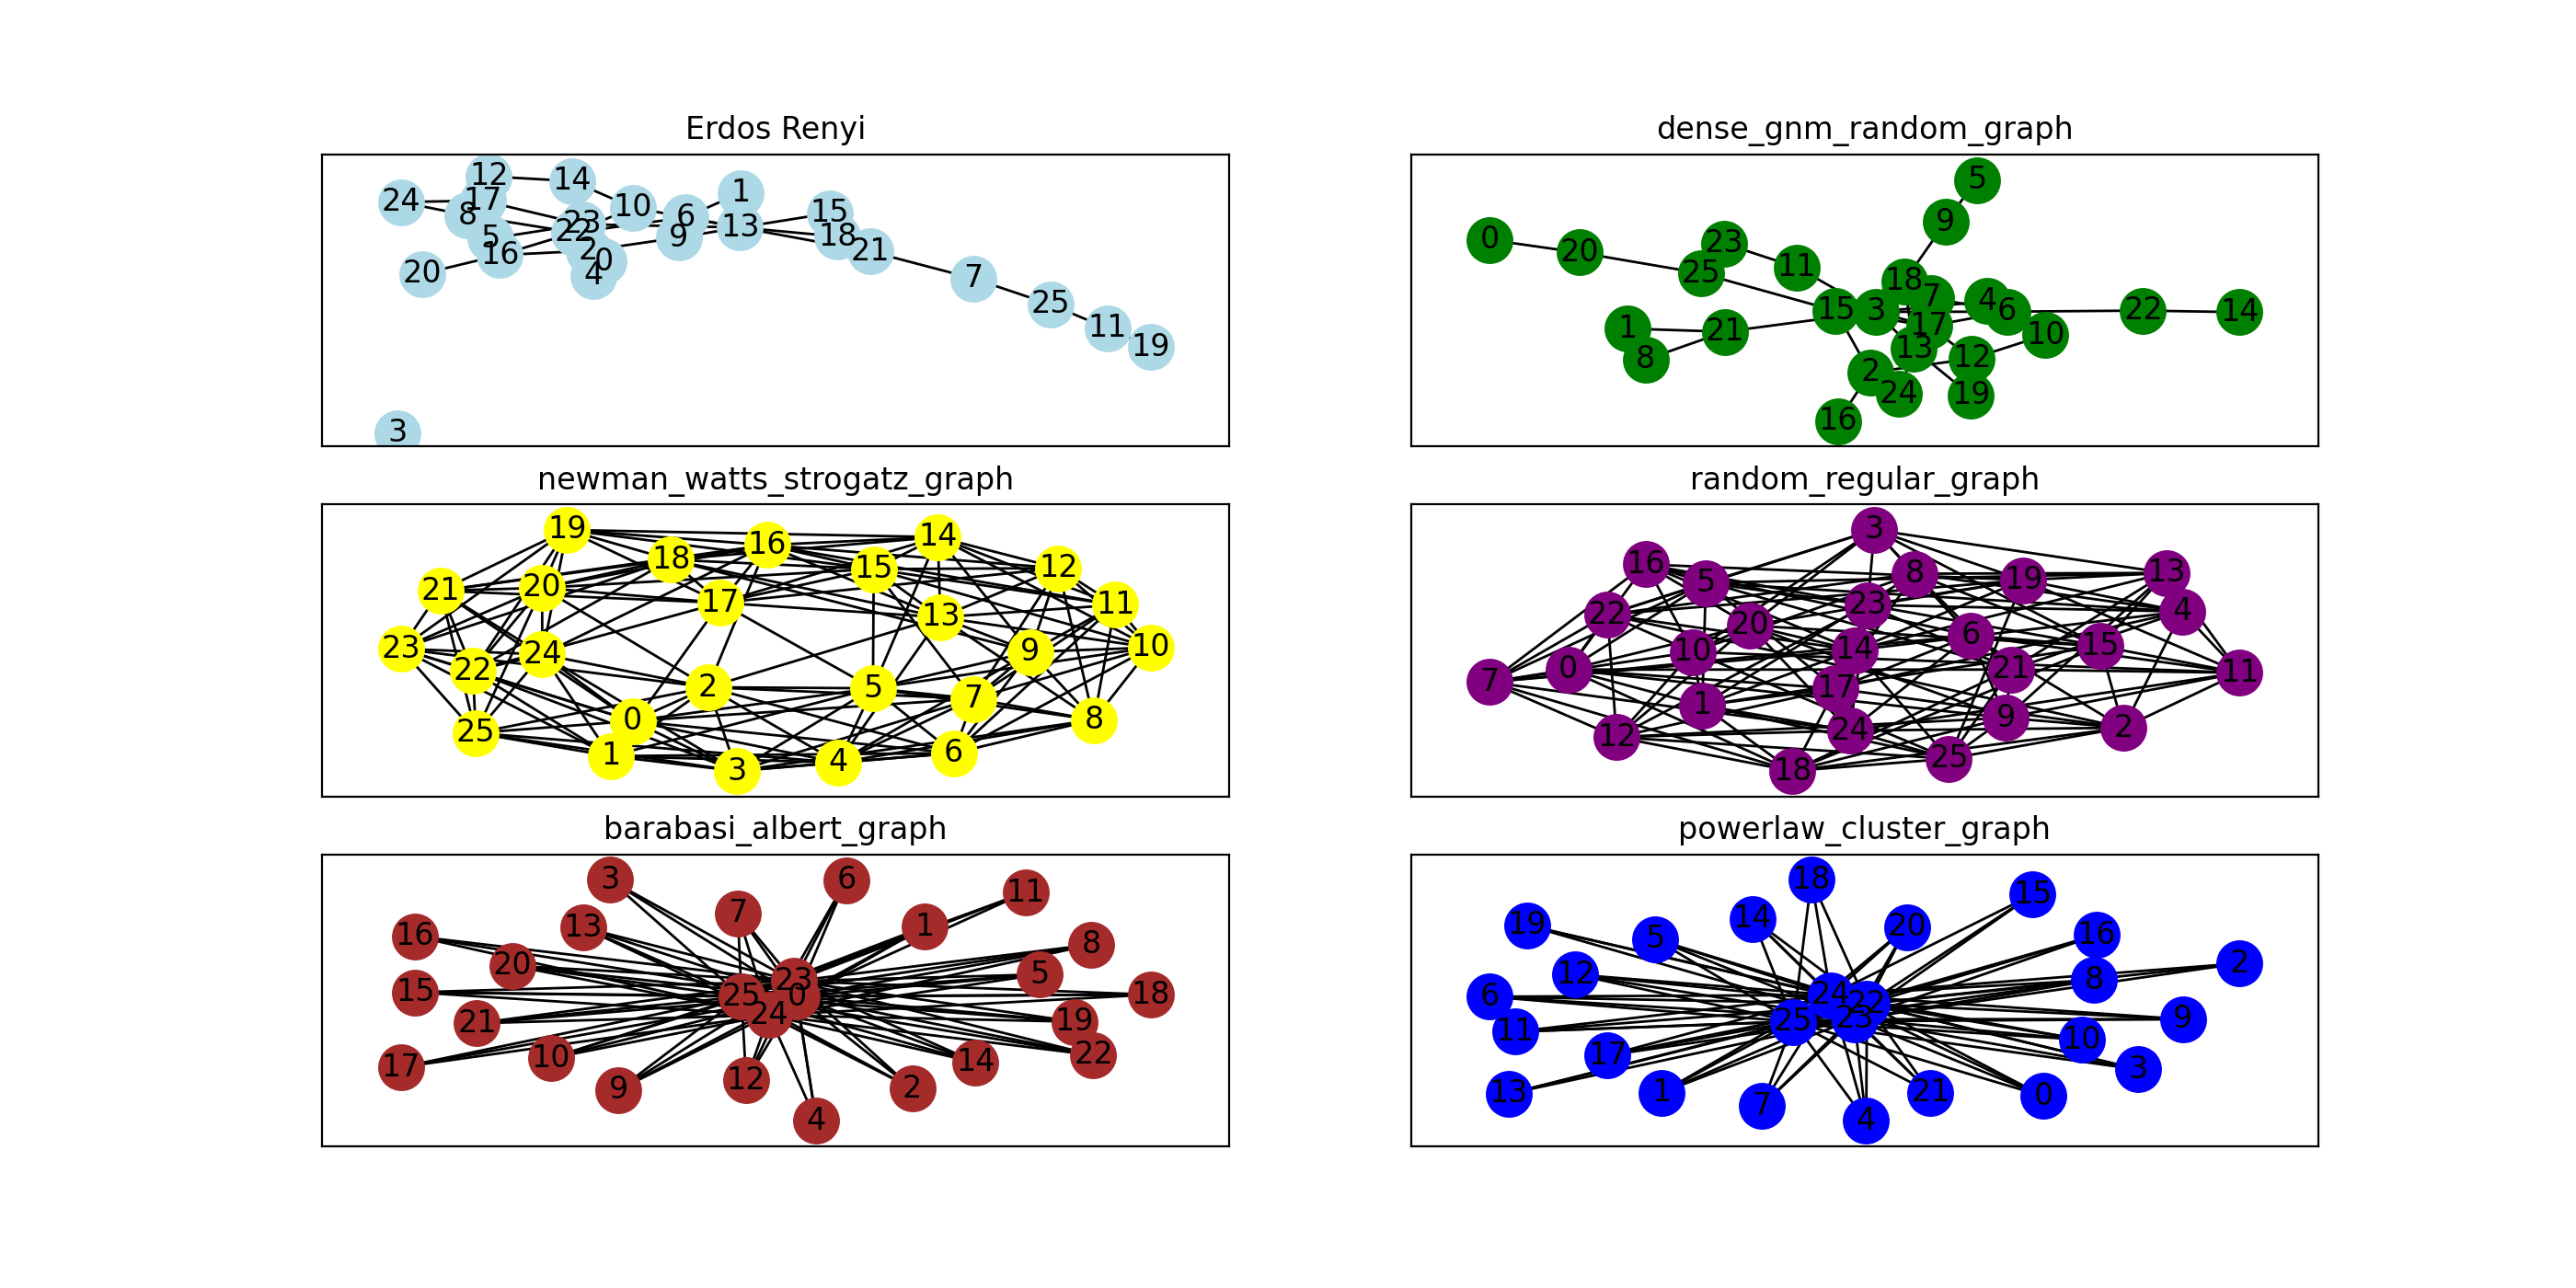
\includegraphics[width=1.2\textwidth]{Graphics/6Random.png}
    \caption{Zufällig erstellte Graphen mit 25 Knoten entsprechend der jeweiligen Methoden}
    \label{RandomGraphen}
\end{figure}
\newpage

Bei den Graphen in Abbildung \ref{RandomGraphen} wurde lediglich eine visuelle Interpretation durchgeführt und nicht die Graphen mit den jeweiligen Zentralitäten analysiert. Auf den ersten Blick erkennen wir, dass bei allen sechs Modellen Unstimmigkeiten zu typischen Kriterien von \textit{sozialen Netzwerken} aus Tabelle \ref{TableEigenschaften} auftreten. Beispielsweise bei dem \textit{Barabasi Albert Graph} und dem \textit{Powerlaw cluster graph} (\textbf{5} und \textbf{6}) sind einzelne zentrale Knoten zu erkennen. Diese zentrale Knoten sind von vielen weiteren Knoten umgeben, die alle wiederum mit diesen zentralen Knoten verbunden sind. Es sind also keine Cliquen und auch keine Cluster zu erkennen. Auch der \textit{newman watts strogatz graph} und der \textit{random regular graph} (\textbf{3} und \textbf{4}) entsprechen nicht den erwünschten \textit{sozialen Netzwerken}. Bei beiden Plots scheint es, als sei jeder Knoten mit jedem weiteren Knoten verbunden, was erneut eine untypische Eigenschaft ist. Es existiert also nur lediglich eine große Clique. Nun bleiben noch die beiden Plots des \textit{Erdos Renyi-Graphen} und \textit{dense gnm random graph} (\textbf{1} und \textbf{2}), welche ebenfalls nicht unseren Erwartungen entsprechen. Der Plot des \textit{dense gnm radom graph} weist zwar einzelne Äste auf, doch generell wenige Cliquen enthalten und keine Cluster aufweist, weshalb dieses Modell ebenfalls nicht brauchbar ist. Bei dem \textit{Erdos Renyi Modell} besteht die gleiche Problematik wobei hier noch das Problem hinzu kommt, dass ein isolierter Knoten existiert. Ein isolierter Knoten ist ein Knoten der keinen Nachbarn besitzt, also Grad $0$ aufweist.
Dies würde beispielsweise auf Sozial Media, bezogen bedeuten, dass Nutzer*innen auf dieser Plattform angemeldet sind, die keinerlei Verbindungen besitzen. Dies kann durchaus der Fall sein, es ist aber sehr unwahrscheinlich, dass Menschen auf solchen Plattformen angemeldet sind und keinerlei Freunde haben oder andere Nutzer*innen folgen.
\newpage
Schließlich kommt bei den oberen zwei Modellen noch dazu, dass bereits visuell betrachtet kaum Cliquen und auch keine Brücken auffindbar sind. Deshalb muss auch bei diesem Modell kritisch hinterfragt werden, ob es sich bei den Graphen um ein \textit{typisches soziales Netzwerke} handeln könnte. Deshalb liegt nahe, dass Anpassungen durchgeführt werden müssen.\\


Eine mögliche Adaption wird erzielt, indem von den zufälligen Graphen-Methoden, die im vorherigen Abschnitt eingeführt wurden, abgewichen wird. Eine weitere Überlegung wäre, alle Formeln selbständig zu implementieren und nicht die bereits vordefinierten Funktionen zu verwenden. Zum Einen sind diese vordefinierten Funktionen intransparent und daher auch fehleranfälliger, aber auch der Zugriff auf diese ist nicht ganz einfach. \\
Für die Generierung eines \textit{sozialen Netzwerks} wird unter anderem eine Methode benötigt, die einzelne zufällige Graphen erstellt. Diese zufälligen Graphen sollen am Ende die jeweiligen Cluster darstellen, welche durch Brücken miteinander verbunden sind. Dadurch wären die ersten Kriterien eines typischen sozialen Netzwerks aus Tabelle \ref{TableEigenschaften} erfüllt.

\begin{algorithm}
\caption{Random Adjazenzmatrix}\label{randomAdjacency}
\begin{algorithmic}[1]
\Procedure{random adjacency matrix}{}
\State $\textit{matrix} \gets \text{zufällige Matrix der Größe (n,n) zufällig befüllt mit Werten zwischen 0 und 1}$
\For {alle \textit{i} in matrix}
\State befülle die Diagonale der Matrix mit 1
\For {alle \textit{i und k} in matrix}
\State setze die Wahrscheinlichkeit \textit{prob} auf einen zufälligen Wert zwischen 0 und 1
\If{\textit{matrix} an der Stelle [i][k] größer als \textit{prob}}
\State setze \textit{matrix} an dieser Stelle auf 0
\Else 
\State setze diese Stelle auf 1
\EndIf
\EndFor
\EndFor
\For {alle \textit{i} in \textit{matrix}}
\State was für \textit{matrix} an der Stelle [i][j] gilt, muss auch für [j][i] gelten
\State \textbf{RETURN} \textit{matrix}
\EndFor
\EndProcedure
\end{algorithmic}
\end{algorithm}

Der Algorithmus \ref{randomAdjacency} erstellt zufällige Matrizen, die aber erst noch zu einer großen Matrix zusammengefügt werden müssen. Die zufälligen einzelnen Matrizen sind die Cluster beziehungsweise Teilgraphen des sozialen Netzwerks. Doch wollen wir diese Cluster nun zu einem großen Graphen beziehungsweise einer großen Matrix zusammenführen. Hierfür benötigt man die Methode \textit{Graph appender}. Der Algorithmus \ref{GraphAppender} dieser Methode soll wie folgt aussehen: 

\begin{algorithm}
\caption{alle Subgraphen zu einer Liste zusammenführen}\label{GraphAppender}
\begin{algorithmic}[1]
\Procedure{graph appender}{}
\State $\textit{graphs} \gets \text{leeres Array}$
\State $\textit{n} \gets \text{Anzahl an Subgraphen / Matrizen}$
\For {alle \textit{i} zwischen 1 und \textit{n}}
\State $\textit{k} \gets \text{zufälliger integer, Größe des Subgraphen}$
\State \textbf{goTo} \text{Algorithm 1 mit dem übergebenen Wert \textit{k}}
\State \text{füge random Matrix in \textit{graphs} ein} 
\State \textbf{RETURN} \textit{graphs}
\EndFor
\EndProcedure
\end{algorithmic}
\end{algorithm}

\newpage
Die einzelne Matrizen werden der dynamischen Datenstruktur (Liste) hinten angehängt.
Nachdem nun eine Liste mit vielen zufällig erzeugten Matrizen generiert ist, fehlt lediglich eine Methode, um die Graphen zusammenzuführen und sicherzustellen, dass die Teilgraphen miteinander durch Brücken verbunden sind. Wir wollen also insgesamt sicherstellen, dass durch die Algorithmen \ref{randomAdjacency}, \ref{GraphAppender} und \ref{uniteGraphs} einzelne zufällige Subgraphen erstellt werden, die mithilfe des \textit{graph appenders} zu einer Liste zusammengeführt werden und nun über Brücken Verbindungen zueinander gebildet werden. Der Algorithmus \ref{uniteGraphs} sieht wie folgt aus:

\begin{algorithm}
\caption{Graphs zusammenführen}\label{uniteGraphs}
\begin{algorithmic}[1]
\Procedure{unite graphs}{}
\State $\textit{graphs} \gets \text{Graph aus Algorithm \ref{GraphAppender}}$
\If {\text{\textit{graphs} aus nur einem Element besteht}}
\State \text{gebe \textit{graphs} zurück}
\EndIf
\State $\textit{dim} \gets \text{0}$
\State $\textit{big graph} \gets \text{Graph mit Nullen befüllt}$
\For{alle \textit{i} zwischen \textit{0} und der Länge von \textit{graphs}}
\State $\textit{Variable a} \gets \text{zufälliger integer zwischen 0 und Länge von graphs}$
\State $\textit{Variable b} \gets \text{zufälliger integer zwischen 0 und Länge von graphs}$
\For{alle \textit{j und k} zwischen \textit{0} und \textit{graphs}}
\State $\textit{l} \gets \text{summierte Länge von \textit{graphs} bis zur Stelle i}$
\State $\textit{graph} \gets \text{\textit{graphs} an der Stelle \textit{i}}$
\\
\State $\text{in den Zeilen 16 und 17 werden die einzelnen Cluster in \textit{big graph} eingefügt}$
\\
\State $\text{\textit{big graph} an der Stelle [(l+j)][(l+k)]} \gets \text{graph[j][k]}$
\State $\text{\textit{big graph} an der Stelle [(l+k)][(l+j)]} \gets \text{graph[k][j]}$
\\ 
\State $\text{in den Zeilen 21 und 22 werden die einzelnen Cluster durch Brüken verbunden}$
\\
\State $\text{\textit{big graph} an der Stelle [(l+a)][(l+b+graphs Länge an [i]) modulo dim]} \gets \text{1}$
\State $\text{\textit{big graph} an der Stelle [(l+b+graphs Länge an [i]) modulo dim)][(l+a)]} \gets \text{1}$
\EndFor
\EndFor
\\
\\
\textit{nun wird der Knoten mit der höchsten Gradzentralität gesucht}\\
\State $\textit{counter 1} \gets \text{0}$
\State $\textit{counter 2} \gets \text{0}$
\State $\textit{Knoten} \gets \text{0}$
\For{\textit{i und j} zwischen \textit{0} und der Länge von \textit{graphs}}
\If{\textit{graphs} an der Stelle [i][j] ungleich \textit{0}}
\State $\textit{counter 1} \gets \text{erhöhe um 1}$
\If{\textit{counter 1} größer \textit{counter 2}}
\State $\textit{counter 1} \gets \text{counter 2}$
\State $\textit{Knoten} \gets \text{i}$
\EndIf
\EndIf
\EndFor
\textbf{RETURN} \textit{Knoten}
\EndProcedure
\end{algorithmic}
\end{algorithm}

\newpage
Jetzt ist ein großer Graph generiert, bestehend aus vielen zufälligen kleinen Graphen, welche durch den Knoten mit den meisten ein- und ausgehenden Kanten mit einem weiteren Subgraphen verbunden sind. Dieses Vorgehen ist aber nicht in einem der drei Algorithmen \ref{randomAdjacency}, \ref{GraphAppender} oder \ref{uniteGraphs} beschrieben, sondern im Git Repo \cite{TZ} zu finden. 
Nach weiteren Überlegungen, wie es möglich wäre, den generierten Graph noch mehr sozialen Netzwerken ähneln zu lassen und die Kriterien aus Tabelle \ref{TableEigenschaften} zu erfüllen, ist zusätzlich die Idee entstanden eine Methode zu schreiben, die sicherstellt, dass der generierte Graph aus einer bestimmten Anzahl an Cliquen besteht. Mit diesem zusätzlich Faktor soll sichergestellt werden, dass der generierte Graph mehr Kanten besitzt als davor, um die Wahrscheinlichkeit für eine existierende Clique zu erhöhen. Der Cliquen-Methode, die ebenfalls im Git Repo \cite{TZ} zu finden ist, soll hierfür eine fixe Zahl $n$ übergeben und zusätzlich sichergestellt werden, dass stetig neue Graphen generiert werden, bis die Anzahl an Cliquen genau der fixen Zahl $n$ entspricht.
Durch die Algorithmen \ref{randomAdjacency}, \ref{GraphAppender} und \ref{uniteGraphs} entsteht schließlich folgender Graph:

\FloatBarrier
\begin{figure}[h!]
    \centering
    \hspace*{-1.5cm}
    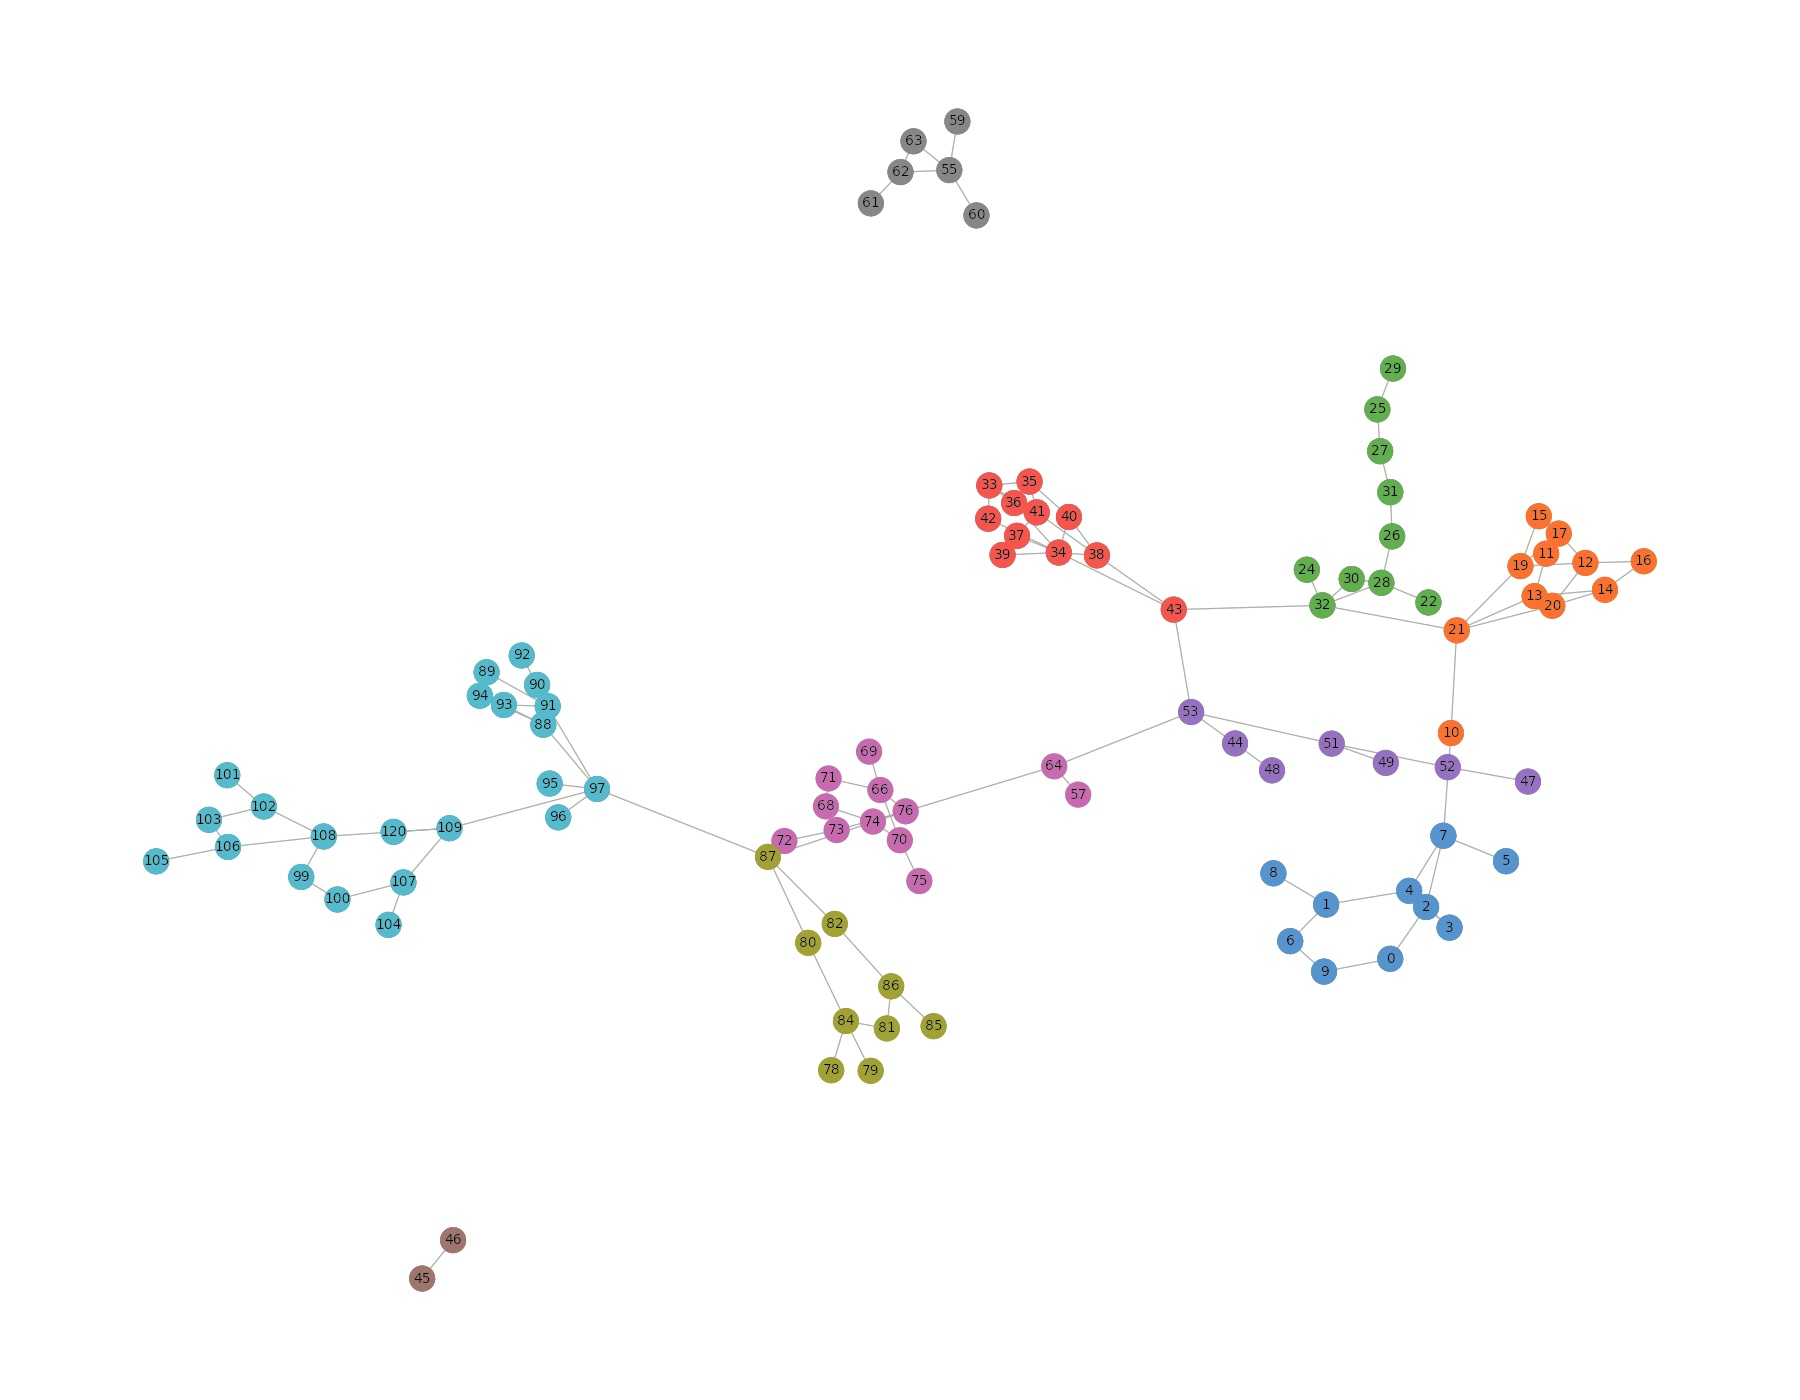
\includegraphics[width=1.0\textwidth]{Graphics/NearSocialNetwork.jpg}
    \caption{Zufälliger sozialer Graph mit höchster Grad-Zentralität als Verbindungsknoten }
    \label{NearSozialerGraph}
\end{figure}

\newpage
Nachdem Abbildung \ref{NearSozialerGraph} visuell betrachtet durchaus \textit{Sozialen Netzwerken} ähnelt, muss noch eine weitere Verbesserung durchgeführt werden. Bei einer genaueren Betrachtung der Abbildung fällt auf, dass die Teilgraphen wenige Verbindungen, Brücken, untereinander aufweisen. Dies liegt an der Idee von Algorithmus \ref{uniteGraphs}, den Knoten mit der höchsten Gradzentralität zu wählen und diesen dann mit einer beliebigen weiteren Gruppe zu verbinden. Doch in der Realität ist ein solches Phänomen sehr unwahrscheinlich und erfüllt nicht die Bedingungen aus Tabelle \ref{TableEigenschaften} für ein typisches soziales Netzwerk. Denn dies würde beispielsweise heißen, dass an der Universität Ulm alle Student(en)*innen der Fakultät für Ingenieurwissenschaften, Informatik und Psychologie untereinander in einer Weise miteinander verbunden sind, jedoch nur die Professor(en)*innen, welche die höchste Gradzentralität aufweisen, mit eine*m/r weiteren Professor*in einer anderen Fakultät verbunden sind. Dies ist aber nicht realistisch wenn bedacht wird, dass auch beispielsweise Student(en)*innen der Fakultät für Mathematik und Wirtschaftswissenschaften durchaus Kontakte zu der Fakultät für Ingenieurwissenschaften, Informatik und Psychologie haben können oder auch mit den jeweiligen Professor(en)*innen. Dementsprechend muss dieses Kriterium ebenfalls in der Implementierung berücksichtigt werden. Das kann gewährleistet werden, indem jedem Knoten eine zufällige Wahrscheinlichkeit zugeschrieben wird, die angibt, ob eine Kante zwischen den Clustern oder Subgraphen existiert. Hierfür wird der Algorithmus \ref{uniteGraphs} ab Zeile \textit{17} ersetzt zu:

\begin{algorithm}
\caption{Verbindung Subgraphen}\label{connection}
\begin{algorithmic}[1]
\Procedure{connection subgraphs}{}
\State $\textit{prob} \gets \text{zufällige Zahl, die sehr klein ist}$
\For {alle \textit{i und j} liegen in der Matrix big graph}
\State \textit{befülle die Diagonale der Matrix mit 0}
\EndFor
\For {alle \textit{i und k} liegen in der Matrix}
\State $\textit{variable} \gets \text{zufällige Zahl zwischen 0 und 1}$
\If{\textit{variable} kleiner \textit{prob}}
\State \textit{setze big graph [i][k] auf 1}
\EndIf
\EndFor
\EndFor
\textbf{RETURN} big graph
\EndProcedure
\end{algorithmic}
\end{algorithm}

Mit Algorithmus \ref{connection} kann sichergestellt werden, dass die Subgraphen vermehrt miteinander verbunden sind und nicht von dem Knoten mit der höchsten Gradzentralität abhängen. Dadurch ist ein weiteres Kriterium aus Tabelle \ref{TableEigenschaften} bezüglich der Existenz von mehreren Brücken, erfüllt.

\section{Die Analyse des generierten Graphen}
Mit den Überlegungen aus dem vorherigen Kapitel und den dort erläuterten Methoden, lassen sich \textit{typische soziale Netzwerke} nach den Kriterien aus Tabelle \ref{TableEigenschaften} generieren. Um zu beweisen, dass es sich tatsächlich um ein typisches Netzwerk handelt, soll ein neues generiert und eine Analyse damit durchgeführt werden. Ziel ist es zu zeigen, dass die mit dem Generator erzeugten Graphen tatsächlich näherungsweise \textit{sozialen Netzwerken} entsprechen, welche die Bedingungen aus Tabelle \ref{TableEigenschaften}.

\FloatBarrier
\begin{figure}[h!]
    \centering
    \hspace*{-2cm}
    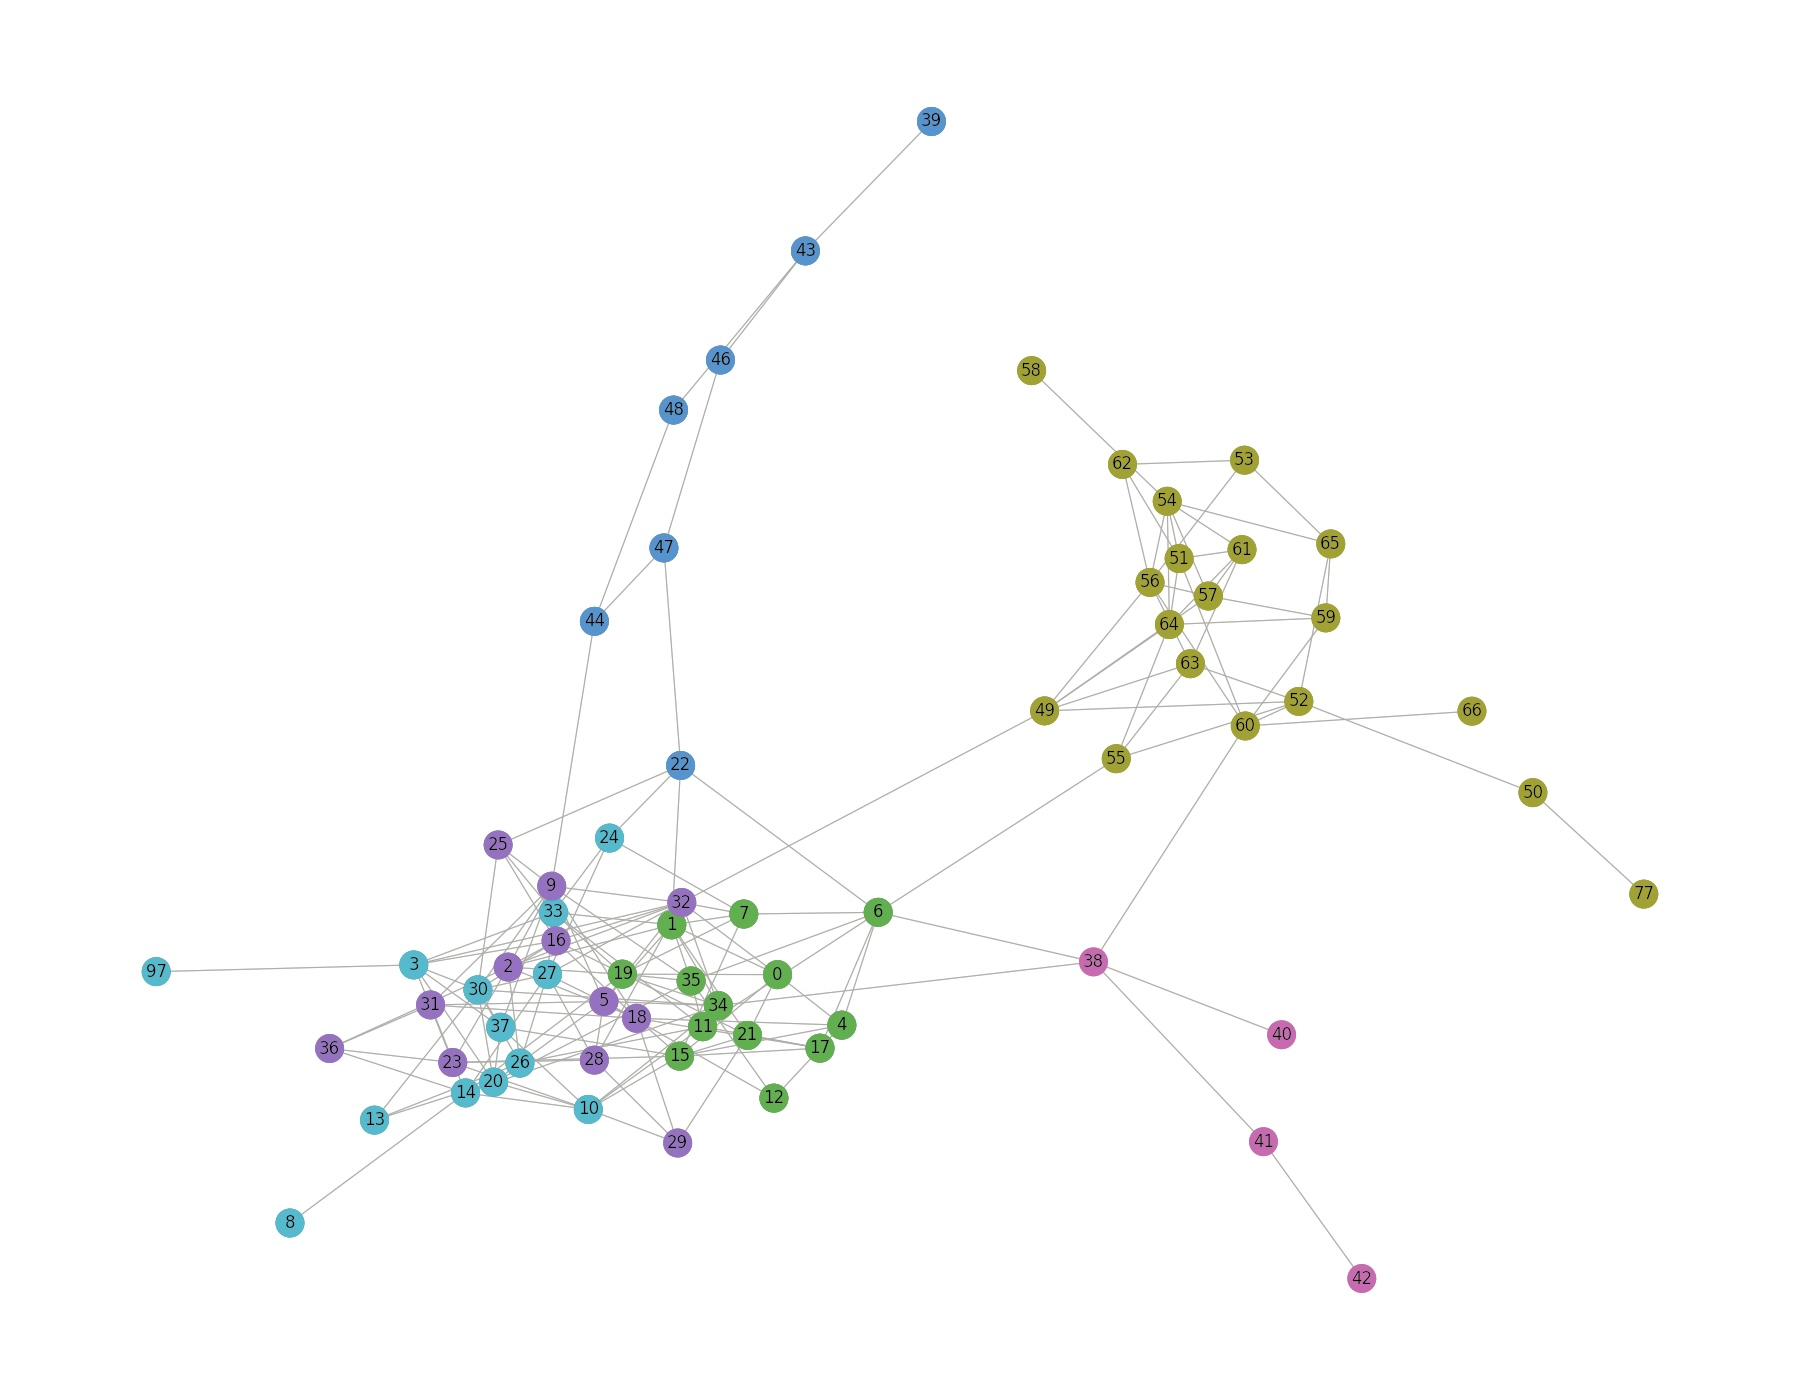
\includegraphics[width=0.7\textwidth]{Graphics/Random_moreConnections.jpg}
    \caption{Zufälliges soziales Netzwerk mit realistischeren Verbindungen}
    \label{fig:SNA}
\end{figure}

\FloatBarrier

Bei der visuellen Betrachtung der Abbildung \ref{fig:SNA} ähnelt die Struktur auf jeden Fall der, eines sozialen Netzwerks, siehe beispielsweise Abbildung \ref{fig:GameOfThrones}. Doch um eine fundierte Aussagen treffen zu können, müssen auch die Zentralitäten genauer analysiert werden. Hierfür wird folgende Tabelle verwendet:

\begin{table}[h!]
\footnotesize
\caption{Werte oberer Graph}
\begin{tabular}{lcccc}\toprule 
\textbf{Knoten} &\textbf{Grad-Zentr.} &\textbf{Nähe-Zentr.}  &\textbf{Between-Zentr.} \\
 &\\\midrule
  1 & 0.149254  & 0.389535 & 0.0429244   \\
  2 & 0.134328  & 0.370166 & 0.0366434   \\
  3 & 0.119403  & 0.350785 & 0.0516569   \\
  5 & 0.119403  & 0.378531 & 0.0341306   \\
  6 & 0.119403  & 0.385057 & 0.145038    \\
  7 & 0.0895522 & 0.358289 & 0.0208983   \\
 10 & 0.119403  & 0.341837 & 0.0240985   \\
 11 & 0.104478  & 0.360215 & 0.0212421   \\
 14 & 0.119403  & 0.3350    & 0.0454434   \\
 18 & 0.134328  & 0.340102 & 0.0283754   \\
 22 & 0.0746269 & 0.348958 & 0.0740623   \\
 27 & 0.119403  & 0.360215 & 0.0342121   \\
 30 & 0.149254  & 0.348958 & 0.0412278   \\
 32 & 0.179104  & 0.435065 & 0.266448    \\
 34 & 0.134328  & 0.394118 & 0.112543    \\
 35 & 0.104478  & 0.362162 & 0.0290967   \\
       
  \\\bottomrule
 \end{tabular}
  &
\begin{tabular}{lccc}
\toprule 
\textbf{Knoten} &\textbf{Grad-Zentr.} &\textbf{Nähe-Zentr.}  &\textbf{Between-Zentr.}\\
   &\\\midrule
 38 & 0.0746269 & 0.36612  & 0.154688    \\
 41 & 0.0298507 & 0.271255 & 0.0298507   \\
 43 & 0.0447761 & 0.198813 & 0.030303    \\
 44 & 0.0447761 & 0.295154 & 0.0773717   \\
 46 & 0.0298507 & 0.219672 & 0.0205638   \\
 47 & 0.0447761 & 0.27459  & 0.0520902   \\
 48 & 0.0298507 & 0.232639 & 0.0373285   \\
 49 & 0.0895522 & 0.36413  & 0.221288    \\
 50 & 0.0298507 & 0.241877 & 0.0298507   \\
 52 & 0.0895522 & 0.314554 & 0.0885577   \\
 54 & 0.104478  & 0.254753 & 0.0327816   \\
 55 & 0.0597015 & 0.325243 & 0.0670173   \\
 56 & 0.104478  & 0.303167 & 0.0672381   \\
 57 & 0.0746269 & 0.290043 & 0.0213757   \\
 60 & 0.0895522 & 0.313084 & 0.0903114   \\
 64 & 0.0895522 & 0.304545 & 0.0530434   \\
      \\\bottomrule
\end{tabular}
\end{table}
\label{TablleSNA}

\FloatBarrier
Bei dieser Tabelle handelt es sich um die \textbf{32} wichtigsten Knoten. Denn alle diese Knoten weisen eine höhere \textit{Zwischen-Zentralität} als \textbf{0.02} auf. Dieser Wert entspricht ungefähr dem Mittelwert aller berechneten Zentralitäten. Die andern Knoten sind außen vor gelassen, da sie in Relation gesehen eher unwichtig für das Netzwerk sind.
Bei der \textit{Grad-Zentralität} aus der Tabelle \ref{TablleSNA} sehen wir, dass die meisten Knoten einen Wert höher als \textbf{0.1} aufweisen. Zudem weisen einige, wenige Knoten eine \textit{Grad-Zentralität} höher als \textbf{0.13} auf. Genau genommen handelt es sich hier um Knoten \textbf{1} mit einem Wert von \textbf{0.149254}, Knoten \textbf{2} mit dem Wert \textbf{0.134328}, Knoten \textbf{18} mit dem Wert \textbf{0.134328}, Knoten \textbf{30} mit einer Zentralität von \textbf{0.149254}, zudem um Knoten \textbf{32} mit dem höchsten Wert von \textbf{0.179104} und schließlich Knoten \textbf{34} mit einer \textit{Grad-Zentralität} von \textbf{0.134328}. \\

Die aufgezählten Knoten sind, den Werten zu urteilen nach, zentral wichtig für den Graphen und befinden sich höchstwahrscheinlich, visuell gesehen, im Zentrum des Graphen in Abbildung \ref{fig:SNA}. Bei der visuellen Analyse, kann diese Behauptung teilweise bestätigt werden, denn diese Knoten fallen direkt auf. Ein hoher Zentralitätswert bei einem Knoten sagt aus, dass es sich beispielsweise im realen Leben um eine vermutlich sehr berühmte / bekannte Person handeln wird. Daher besteht die Annahme, dass es sich bei diesem Knoten, würde er auf die Realität bezogen betrachtet werden, beispielsweise um einen Star, einen Influenzer oder eine, auf weitere Arten bekannte Person handelt. Doch ebenso ist es möglich, dass die Person viele weitere Personen kennt, oder von vielen weiteren Personen gekannt wird. Wichtig ist, dass nicht nur die Grad-Zentralität eine zentrale Rolle für die Analyse spielt. Im Weiteren betrachten wir auch die \textit{Nähe-Zentralität}. Doch um auch bei diesem Aspekt nicht alle \textbf{32} Werte aufzuzählen, werden im Folgenden nur Knoten betrachtet, die einen Wert höher als \textbf{0.37} aufweisen, da es sich dabei erneut um einen guten Mittelwert handelt. Diesen Grenzwert übertrifft der Knoten \textbf{1} mit einem Wert von \textbf{0.389535}, Konten \textbf{2} mit dem Wert \textbf{0.370166}, zudem Knoten \textbf{5} mit dem Wert \textbf{0.378531}, zusätzlich Knoten \textbf{6} mit der Zentralität \textbf{0.385057}, und schließlich Knoten \textbf{32} mit dem höchsten Wert von \textbf{0.435065} und \textbf{34} mit der Zentralität von \textbf{0.394118}. Laut der Definition aus dem Abschnitt \ref{ch:Zentralitaeten} gilt, je höher die Werte der \textit{Nähe-Zentralität} eines Knoten ist, desto näher befindet sich dieser Knoten zu weiteren Knoten bzw. weist die durchschnittlich kürzesten Wege zu diesen auf. \\

Wird der Graph \ref{fig:SNA} anhand dieser Information betrachtet und werden so die Knoten mit der höchsten \textit{Nähe-Zentralität} gesucht, ist visuell ersichtlich, dass sich diese im gleichen Bereich befinden, wie die Knoten mit der höchsten \textit{Grad-Zentralität}. Die letzte zu untersuchenden Zentralität ist die \textit{Betweenness-Zentralität}. Auch hier betrachtet man wieder die Knoten mit den höchsten Werten, und um nicht alle \textbf{32} Werte aufzuzählen, werden erneut nur Knoten mit einem Wert höher als \textbf{0.09} ausgewählt. Diese Voraussetzung erfüllen neben dem Knoten \textbf{6} mit dem Wert \textbf{0.145038} die Knoten \textbf{32} mit der höchsten Zentralität von \textbf{0.266448} und \textbf{34} mit einem Wert von \textbf{0.112543}, außerdem der Knoten \textbf{38} mit der Zentralität von \textbf{0.154688}, zudem der Knoten \textbf{49} mit dem Wert \textbf{0.221288} und schließlich der Knoten \textbf{60} mit dem Wert \textbf{0.0903114}. 

Das bedeutet für unseren Graphen in Abbildung \ref{fig:SNA}, dass die kürzesten Wege anteilsmäßig am öftesten über diese genannten Knoten verlaufen. Zudem kann vermutet werden, dass es sich bei diesen Knoten um \textit{Brücken} handelt, was der Behauptung aus dem vorherigen Kapitel \ref{ch:CliquenBrücken}, dass es sich bei hohen \textit{Zwischen-Zentralitäten} um \textit{Brücken} handelt, bestätigen würde. Bei der erneuten Betrachtung des Graphen, erkennt man nämlich, dass sich die Knoten in den grün, lila, hellblauen Teilgraphen befinden und links unten zentriert sind. Doch kommt bei der \textit{Zwischen-Zentralität} hinzu, dass sich die Knoten \textbf{49} und \textbf{60} auch im gelbgrünen, rechts oben liegenden, Teilgraphen befinden. Außerdem ist auf den ersten Blick zu erkennen, dass es sich bei den 6 Knoten in Abbildung \ref{fig:SNA} visuell betrachtet, tatsächlich um Brücken handelt. \\

Leider ist an dieser Stelle zu erwähnen, dass die Anzahl an \textit{Cliquen} des Graphen aus der Abbildung \ref{fig:SNA} nicht mehr exakt bekannt ist, da erst nach der weiteren Verbesserung des Codes Rücksicht drauf genommen wurde, die Cliquen-Größe und -Anzahl direkt vorzugeben beziehungsweise der Methode zu übergeben. Daher wird an dieser Stelle nur die Vermutung aufgestellt, dass alle Knoten aus der Tabelle \ref{TablleSNA} Teil von Cliquen sind. Wie viele es jedoch genau sind, lässt sich an dieser Stelle leider nur wage vermuten. Im nächsten Abschnitt wird zusätzlich die Betrachtung der Cliquen des Graphen mit einbezogen. Weitere Zentralitätswerte und Kriterien des Graphen werden an dieser Stelle nicht betrachtet. Nachdem alle Kriterien aus Tabelle \ref{TableEigenschaften} überprüft sind und erfolgreich festgestellt wurde, dass dieser Graph einem \textit{sozialen Netzwerk} ähnelt, wird noch ein weiterer Graph generiert, um sicherzustellen dass es sich nicht um eine zufällige Übereinstimmung handelt. An dieser Stelle soll auch noch ein weiteres Kriterium untersucht werden, nämlich die Verteilung der Zentralitäten.


\newpage
\section{Die Verteilung der Zentralitäten}
Nachdem im vorherigen Kapitel ein erster Versuch unternommen wurde, strukturell \textit{soziale Netzwerke} zu modellieren, soll in diesem Kapitel untersucht werden, ob die klassische Analyse von repräsentativen sozialen Netzwerken für unsere Modelle ähnliche Werte von Zentralitäten erzielt. Das heißt im Konkreten, wir möchten der Frage nachgehen, ob Zentralitätswerte sozialer Netzwerke ähnliche Verteilungen haben. Wenn sich die Vermutung bestätigt, können andere soziale Netzwerke anhand dieses Kriteriums verglichen werden.
Erdös und Renyi (1960), Cliff und Ord (1973) und Friedkin (1981) arbeiteten bereits an Zufallsgraphen und haben die Definition erstellt, dass alle Graphen mit $N$ Knoten und $E$ Kanten dieselbe Wahrscheinlichkeiten haben, ausgewählt zu werden. Ein bekanntes Ergebnis von Erdös und Renyi (1960) ist zudem, dass die Zentralitäten, vor allem aber die Grad-Zentralität, hypergeometrisch verteilt ist, was durch eine Poisson-Verteilung angenähert werden kann \cite{Distribution}. Weitere, vor allem mathematische Beweise, können dem Buch \cite{Distribution} entnommen werden. Im weiteren Teil dieser Arbeit wird demnach untersucht, ob die Verteilungen der Zentralitäten der \textit{Poisson-Verteilung} ähnelt. Zu der Tabelle \ref{TableEigenschaften} kommt also eine weitere Zeile hinzu:

\begin{table}[h!]
\footnotesize
\caption{Weiteres Kriterium eines sozialen Netzwerks}
\label{TableEigenschaften2.0}
\centering
\begin{tabular}{lcc}\toprule 
\textbf{Kriterium} &\textbf{Beschreibung} 
 &\\\midrule
  \textbf{Kriterium 7} & die Zentralitäten eines sozialen Netzwerks sollten \\ &annähernd einer Poisson-Verteilung entsprechen \cite{verteilung} 
  \\\bottomrule
 \end{tabular}
 \end{table}

Da der Graph in Abbildung \ref{fig:SNA} ein zufällig, einmalig erzeugter Graph ist, muss ein neuer Graphen mithilfe des Generators erzeugt werden, um die Verteilung der Zentralitäten zu betrachten. Dies wird sich nicht auf die Untersuchung auswirken, denn die Verteilungen der Zentralitäten unserer Graphen sollte stets gleich oder zumindest ähnlich sein. Bei der erneuten Generierung entsteht nun folgender Graph \ref{fig:distribution} und die zugehörige Verteilung der \textit{Grad-Zentralität}:

\FloatBarrier
\begin{figure}[h!]%
  \centering
  \subfloat[][]{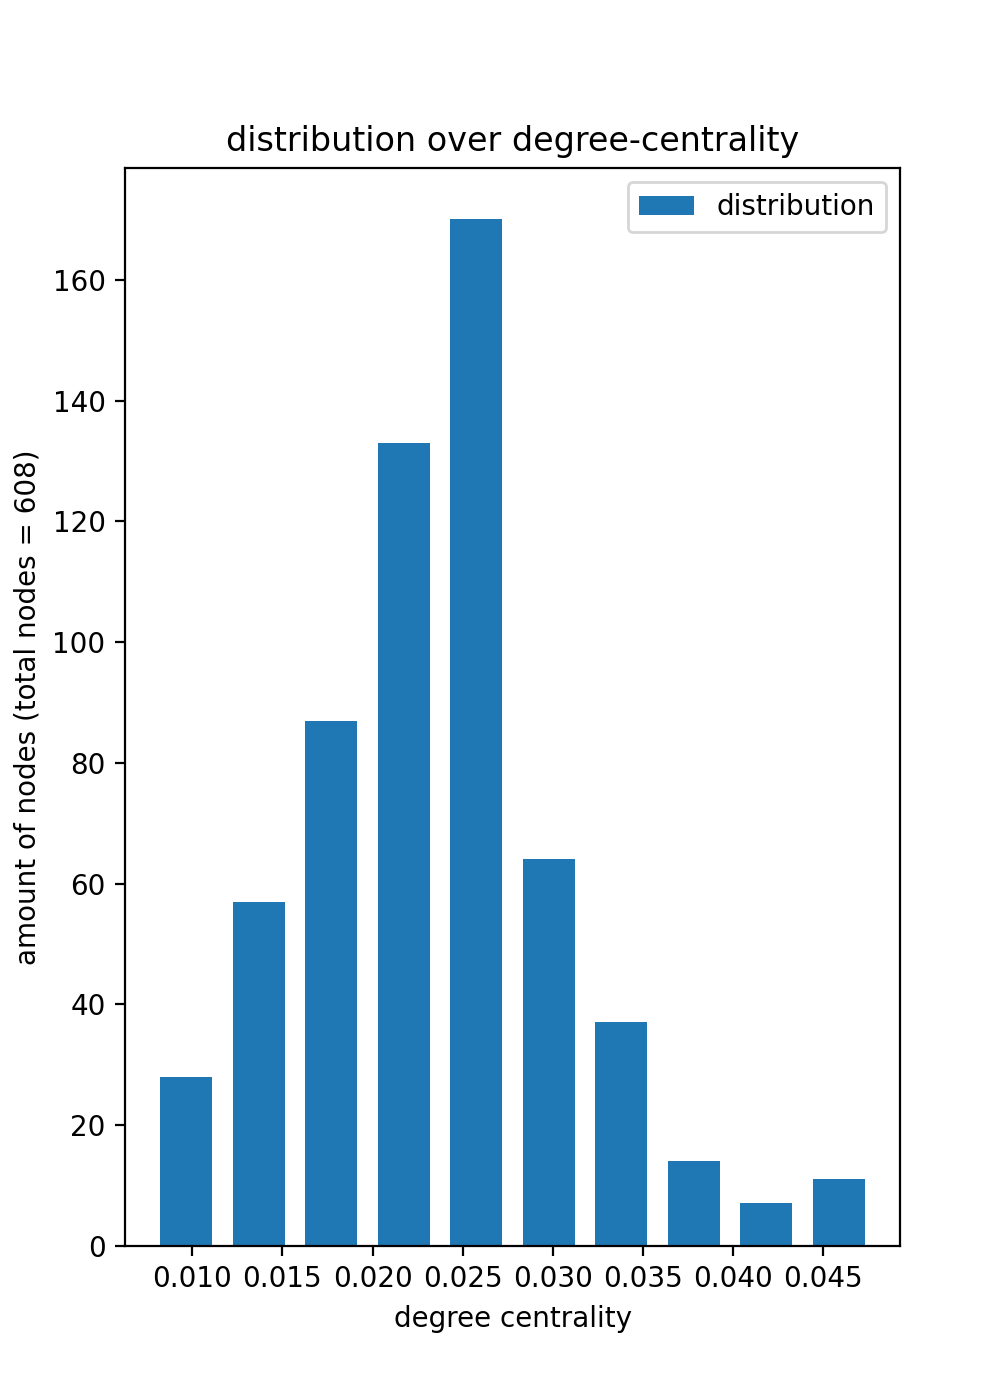
\includegraphics[width=0.4\linewidth]{Graphics/distribution_degree.png}}%
  \qquad
  \subfloat[][]{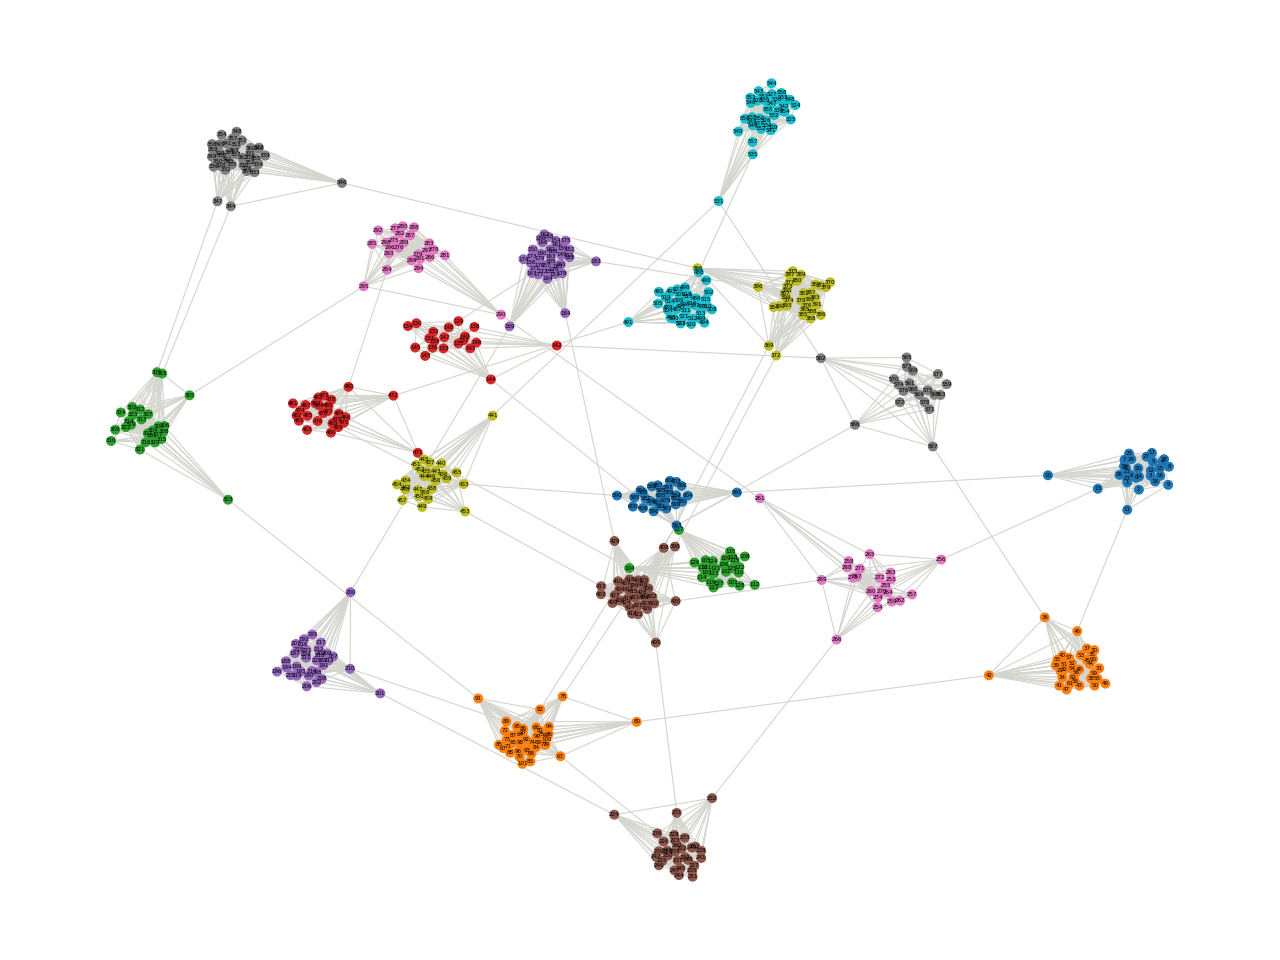
\includegraphics[width=0.5\linewidth]{Graphics/plot_degreeDist.png}}%
  \caption{Verteilung der Grad-Zentralität des Graphen (b)}%
  \label{fig:distribution}
\end{figure}
\FloatBarrier

Es wird ersichtlich, dass die \textit{Grad-Zentralität} normal- beziehungsweise gaußverteilt ist. Natürlich ist zu erwähnen, dass keine perfekte Normal-Verteilung zu sehen ist, sondern eine etwas nach links verschobene Verteilung. Was die möglichen Gründe dafür sind, werden später betrachtet und korrigiert. Diese Verteilung erfüllt tatsächlich die Kriterien aus \\
Tabelle \ref{TableEigenschaften2.0}, denn die Poisson-Verteilung wird für ein größer werdendes $\lambda$ zu einer gaußschen Normalverteilung \cite{Poisson}. Nun ist aber auch noch zu untersuchen, ob sich das Kriterium, der  poisson verteilten Zentralitäten, für die \textit{Nähe-} und \textit{Zwischen-Zentralität} ebenfalls beobachten lässt. Um zusätzlich zu beweisen, dass es sich bei der Gauß-Verteilung der Werte nicht um einen Zufall handelt, wird ein neuer sozialer Graph generiert und die Verteilung der \textit{Grad-}, \textit{Nähe-}, \textit{Zwischen-} und \textit{Eigenvektor-Zentralität} untersucht. Hierbei ist vor allem die Frage, ob die Verteilung dieser einer tatsächlichen Poisson-Verteilung entspricht und falls ja, warum dies der Fall ist, essentiell. Ansonsten wird die Frage gestellt, warum es keiner Poisson-Verteilung entspricht und ob es möglich ist, den Graphen zu verändern um eine solche zu erzielen. Bei der erneuten Generierung entstehen schließlich folgende Plots:

\FloatBarrier
\begin{figure}[h!]%
  \centering
  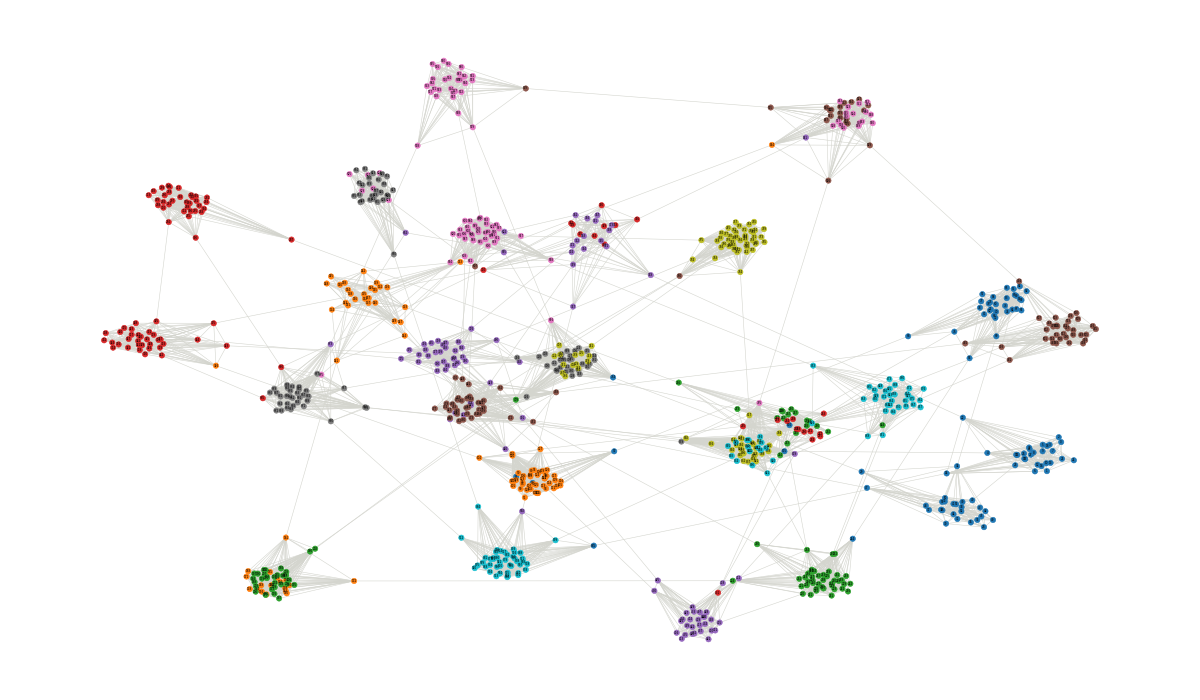
\includegraphics[width=0.7\textwidth]{Graphics/newourSN.png}
  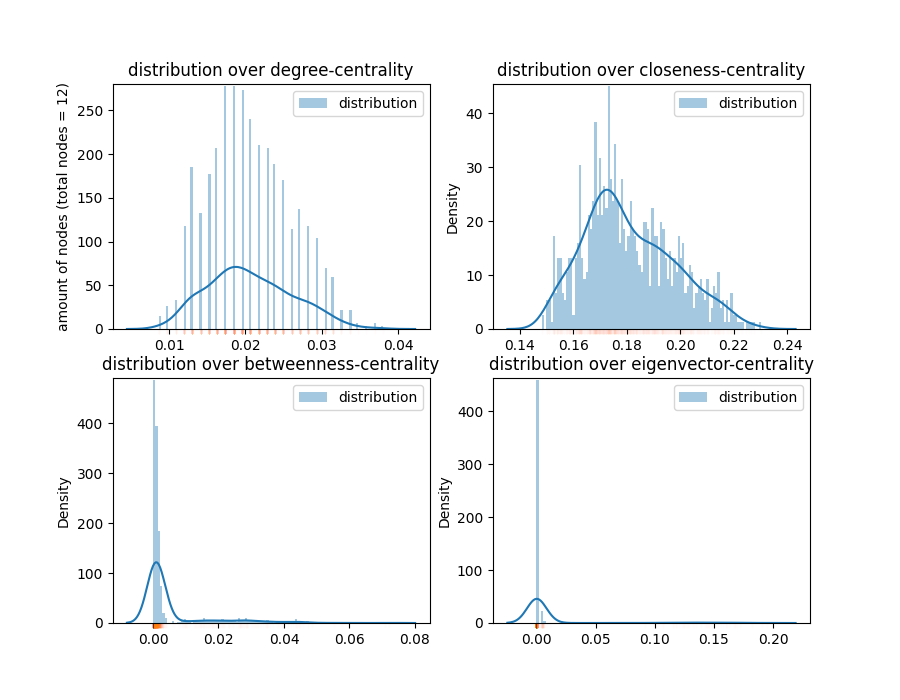
\includegraphics[width=0.9\textwidth]{Graphics/newOurDist.png}
  \caption{Zufälliges soziales Netzwerk und realistischeren Verteilungen}
  \label{fig:distributionALL}
\end{figure}
\FloatBarrier
In der Abbildung \ref{fig:distributionALL} sieht man nun die Verteilungen der Zentralitäten von dem, sich darüber befindenden, sozialen Netzwerks. Die Tabelle mit den Zentralitäts-Werten des Netzwerks befindet sich als Datei in \cite{TZ}. Oben links befindet sich die Verteilung der \textit{Grad-Zentralität}, welche wie bereits zuvor festgestellt, nicht exakt normalverteilt ist, aber Ähnlichkeiten zu erkennen sind und demnach ebenfalls eine annähernde Poisson-Verteilung zu erkennen ist. Vor allem ist auffällig, dass der Balken bei \textbf{0.012} vergleichsweise sehr hoch ist. Über \textbf{50} Knoten weisen diesen Wert auf. Danach geht der darauf folgende Balken nochmals zurück, denn nur noch etwas über \textbf{25} Knoten haben eine Zentralität von circa \textbf{0.03}. Jedoch war zu erwarten, dass sich das Balkendiagramm symmetrisch verhält um der mathematischen Verteilung zu entsprechen, doch das Gegenteil tritt ein. Der genaue Grund hierfür ist mir nicht ersichtlich, aber besteht die Vermutung, dass es nicht weiter schlimm ist und es ausreicht, dass die Verteilungen lediglich annähernd der Poisson-Verteilung entsprechen. Über \textbf{150} Knoten weisen eine Zentralität von \textbf{0.0125} auf, daher sollten auch ebenso viele den Wert \textbf{0.025} besitzen. Hingegen ist positiv hervorzuheben, dass genau \textit{ein Peak} erreicht wurde, wie auch zu erwarten war, um der mathematischen Verteilung zu entsprechen. Außerdem sind alle Balken vor dem Peak kontinuierlich aufsteigend und nach dem Peak kontinuierlich absteigend. Doch lediglich eine Unstimmigkeit sticht hier heraus, bei dem Zentralitätswert von \textbf{0.0357} den etwas unter \textbf{25} Knoten besitzen. Fraglich ist hier, warum der Balken erneut höher ist als sein Vorgänger. Denn im Regelfall sollten maximal ein bis drei Knoten gefunden werden, die diesen Wert aufweisen. Doch im Allgemeinen erfüllt der Plot genau das Kriterium, das auch zu erwarten ist, nämlich dass die \textit{Grad-Zentralität} annähernd poisson verteilt ist.\\

Das Balkendiagramm der \textit{Nähe-Zentralität} weist einen ähnlichen Verlauf auf wie das der \textit{Grad-Zentralität}. Wir erkennen erneut das erwartete Peak und weitere Balken, die im linken Bereich sehr schnell zum Peak hin ansteigen und rechts vom Peak vergleichsweise langsam abflachen. Auffällig ist erneut, dass der letzte Balken wider Erwartens höher ist als der Balken davor. Eine Aussage, welche auf jeden Fall getroffen werden kann ist, dass es erneut zu Unstimmigkeiten kommt, welche stets an anderen Stellen auftreten und nicht immer denselben Balken betreffen. Doch ist erneut eine Normal Verteilung zu erkennen, die der Poisson Verteilung für hohes $\lambda$ entspricht \cite{Poisson}. Es kann im Allgemeinen zudem angenommen werden, dass je größer der Graph ist, umso eher sind die Zentralitäten von diesem poisson verteilt. Was daran liegt, dass dieser dann mehr Knoten besitzt und diese irgendwann zwangsläufig eine Regelmäßigkeit aufzeigen, da Zahlen in der Mathematik prinzipiell nicht \textit{zufällig}, sondern normalverteilt sind. Grob zusammengefasst, kann die Existenz einer Kante als Binomialverteilung interpretiert werden und diese konvergiert mathematisch gesehen bei einer sehr großen Stichprobe (Anzahl an Knoten in unserem Fall) gegen eine Normal- bzw Gaußverteilung. \\

Bei der \textit{Zwischen-} und \textit{Eigenvektor-Zentralität} sind andere Verteilungen zu erkennen. Zum einen weisen die Balken wenige unterschiedliche Werte auf, zum anderen sind die Ausschläge nicht mehr mittig sondern direkt zu Beginn der Verteilung. Was zunächst verwunderlich erscheint, ist mit einer simplen Erklärung begründet. Die \textit{Nähe-Zentralität} gibt bekanntlich an, wie oft ein Knoten anteilsmäßig bei der Suche nach dem kürzesten Weg durch einen Graphen benutzt wird. Der Ausschlag ist daher die Folge davon, wenn viele kürzeste Wege stets über die gleichen Knoten verlaufen. Das heißt, es existieren keine bis wenige Alternativen und daher verlaufen die kürzesten Wege von beispielsweise Knoten \textbf{1} zu einem weiteren Knoten stets über gleiche, beziehungsweise ähnliche Knoten. Bei der \textit{Eigenvektor-Zentralität} wird zwar die gleiche Beobachtung gemacht, doch sagt diese hier etwas anderes aus. Diese Zentralität gibt eine Einschätzung der Wichtigkeit des Knotens, im Bezug auf seine Nachbarn an, was bezogen auf die Balkendiagramm heißt, dass viele Knoten in diesen Graphen wichtig sind mit Einbeziehung der Nachbarn. Wobei auch vermuten werden darf, dass dies mit der hohen Anzahl an Konten mit höher \textit{Zwischen-Zentralität} zusammenhängt.\newpage
Das heißt im Umkehrschluss wiederum, dass mehr Cliquen im Graph enthalten sind. Tatsächlich sind es \textbf{935} Knoten, \textbf{8952} Kanten und \textbf{10301} Cliquen mit der maximalen Größe von acht Knoten in der Clique.
Die Verteilungen sind dennoch aus der Mathematik bekannt, denn es handelt sich um die \textit{Exponential-Verteilung}, welche ebenfalls in eine \textit{Poisson-Verteilung} übergehen kann. Wie dies genau funktionier, ist \cite{PoissonMathepedia} zu entnehmen.
Danach zu Urteilen handelt es sich bei dem Netzwerk in Abbildung \ref{fig:distributionALL} um ein typisches \textit{soziales Netzwerk} nach Tabelle \ref{TableEigenschaften} und Tabelle \ref{TableEigenschaften2.0}.

\section{Kurzes Recap}
Nachdem zunächst überlegt wurde, wie soziale Netzwerke generiert werden, sind auch gleichzeitig die Probleme der Generierung aufgefallen. Daher wurde der Code fortlaufend verbessert, ein soziales Netzwerk erstellt und danach eine \textit{soziale Netzwerk Analyse} durchgeführt. Schließlich konnte so die Bestätigung erhalten werden, dass die generierten Graphen die Anforderungen eines sozialen Netzwerks aus den Tabellen \ref{TableEigenschaften}, \ref{TableEigenschaften2.0} erfüllt. Danach ist zudem aufgefallen, dass die Zentralitäten regelmäßig sind und eine Poisson-Verteilung nachgewiesen werden kann. Doch muss im Folgenden noch die Frage beantwortet werden, wie die Verteilung der Zentralitäten bei anderen, bereits analysierten, Netzwerken aussieht.

%*****************************************
\chapter{Der Vergleich mit Sozialen Netzwerken}\label{ch:vergleich}
%*****************************************

Im vorherigen Teil der Arbeit haben wir uns damit beschäftigt, wie soziale Netzwerke so gut und realitätsnah wie möglich konstruiert werden können. Wir haben Analysen durchgeführt und festgestellt, dass die Werte unserer \textbf{Grad-} und \textbf{Nähe-Zentralität} näherungsweise normalverteilt sind. Daher liegt es nahe, weitere sozialen Netzwerke und ihre Analysen zum Vergleich heranzuziehen. Leitfragen sind hierbei, was zu erwarten ist, ob die Ergebnisse den Erwartungen entsprechen oder sogar widersprechen und warum dies der Fall ist. Zusätzlich möchten wir optimalerweise eine Möglichkeit erarbeitet, wie wir unsere Graphen bzw. die Generierung angepasst könnten um vielleicht sogar bessere Graphen zu erhalten, die diesen sozialen Netzwerken noch mehr ähneln. 

\section{Der Datensatz und die Analyse}
Auf der Suche nach vergleichbaren sozialen Netzwerken, beziehungsweise Datensätzen, ist die Suche scheinbar endlos. Auf vielen Webseiten sind große Datensätze für alle Nutzer*innen zugänglich. Meistens als \textbf{CSV} Datei, welche ideal zur Erstellung von Plots, über Sozialen Netzwerken, geeignet sind. In diesem Teil der Arbeit betrachten wir mehrere Datensätze. Natürlich aufgrund der Tatsache, dass sie spannend sind aber auch um mehrere Vergleichswerte zu haben. Starten wir zunächst mit den Daten \cite{GOT} von unserem \textbf{Game of Thrones} Plot \ref{fig:GameOfThrones}. Da wir bereit die Analyse der \textbf{Zentralitäten} und die generelle visuelle Analyse des Graphen durchgeführt haben, reicht uns nun lediglich die Verteilung der Zentralitäten durchzuführen. Die Tabelle mit den Werten der Zentralitätsberechnungen befinden sich erneut in \ref{ch:anhang}. Nachdem wir den Datensatz als \textbf{CSV} Datei in Python eingelesen und zunächst den Graphen folgendermaßen konstruiert:

\FloatBarrier
\begin{figure}[h!]%
  \centering
  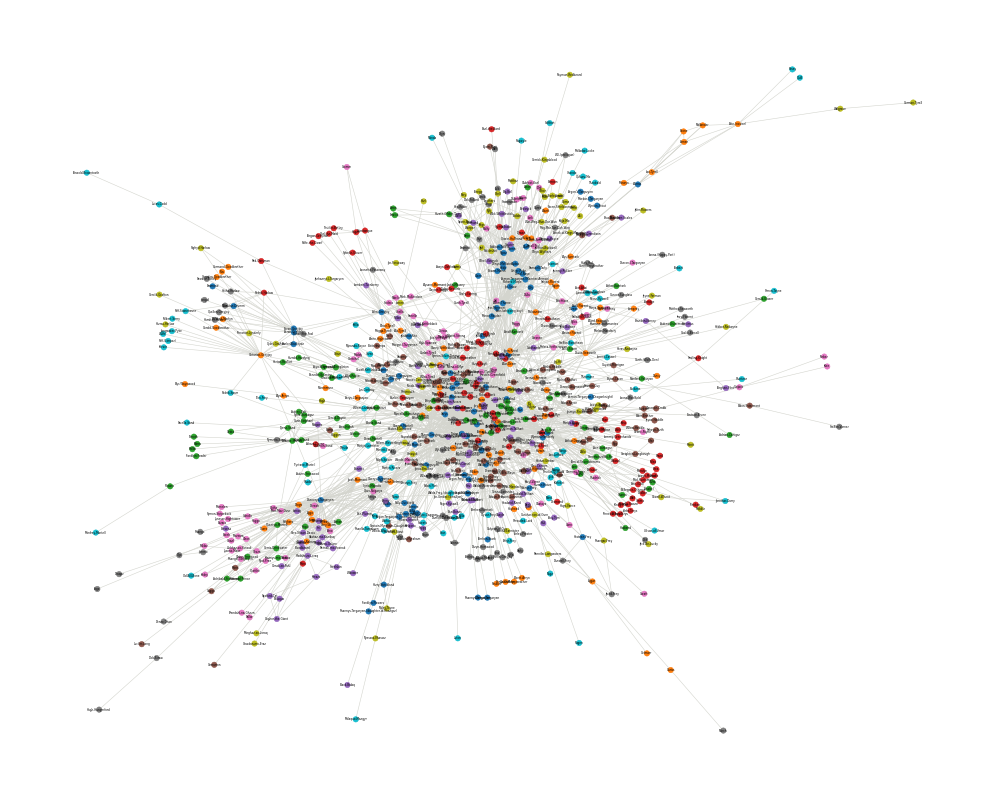
\includegraphics[width=0.5\textwidth]{Graphics/GOTGraph_unweighted.png}
  \caption{Game of Thrones Graph 2.0, \\
  selbst erstellt}
  \label{fig:GOT2.0}
\end{figure}
\FloatBarrier

Dieser Plot ist beabsichtigt klein, da wir ihn lediglich zur Argumentation für die Verteilung der Zentralitäten benötigen und daher die Form des Graphen nur von Bedeutung für uns ist. Zudem ist zu vermerken, dass der eigentliche Datensatz gewichtet ist, und unser Graph daher bereits schon visuell nicht dem Graphen aus \ref{fig:GameOfThrones} ähnelt. Jedoch ist es sinnvoll die Gewichte außen vor zu lassen, da wir in dieser Arbeit ungewichtete Graphen nachbilden. Nachdem wir die Daten des Graphen \ref{fig:GOT2.0} eingelesen, die Zentralitäten berechnet haben und anschließend den Balkengraphen erstellt haben, wurde folgender Plot generiert:

\FloatBarrier
\begin{figure}[h!]%
  \centering
   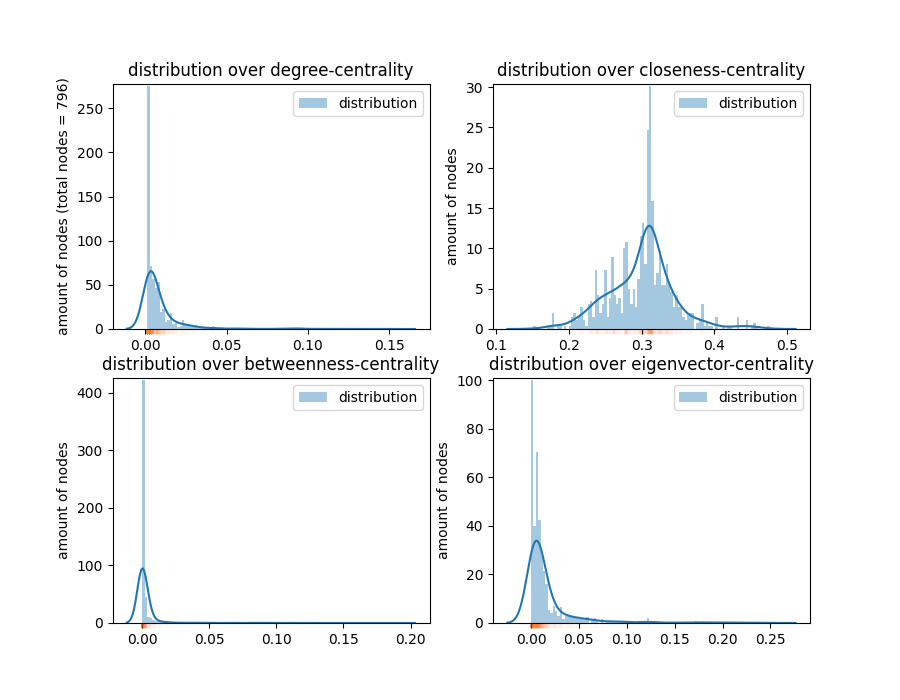
\includegraphics[width=0.8\textwidth]{Graphics/GOTdistribution.png}
  \caption{Game of Thrones Verteilung der Zentralitäten}
  \label{fig:distributionGOT}
\end{figure}
\FloatBarrier
 
 Auf den ersten Blick können wir bereits feststellen, dass wir andere Ergebnisse erwartet haben. Einzig die Verteilung der \textbf{Nähe-Zentralität} ähnelt der erwarteten Normalverteilung. Die \textbf{Betweenness-} und \textbf{Eigenvektor-Zentralität} hingegen ähneln zwar nicht exakt dem, was wir in \ref{fig:distributionALL} herausgefunden haben aber ziehen auf jeden Fall Parallelen. Denn beide haben den Ausschlag im letzten Balken, was wir schon im vorherigen Kapitel damit begründet haben, dass es die Folge davon ist, wenn viele kürzeste Wege stets über die gleichen
Knoten verlaufen, wir also keine Alternativen im Graph haben. Die \textbf{Grad-Zentralität} hingegen darf uns verwundern. Sie ähnelt zum einen stark der Verteilung der \textbf{Eigenvektor-Zentralität} aber keinesfalls der annähernden normalverteilt aus \ref{fig:distributionALL}. Der Ausschlag des letzten Balken ist hingegen schnell erklärt. Wir haben viele Konten, in dem Fall Charaktere, die alle gleich wichtig für den Graphen sind. Diese Konten sind also mit vielen anderen Knoten verbunden, werden daher von vielen anderen Charakteren gekannt oder kennen viele andere Charaktere. Im Allgemeinen sind die Balkendiagramme der \textbf{Zentralitäten} aus \ref{fig:distributionGOT} leider nicht zufriedenstellend. Der Grund, warum die Ergebnisse stark von unseren Erwartungen abweicht ist, dass es sich bei dem Graphen um fiktive Charaktere handelt. Dadurch kann es schnell zu Unstimmigkeiten kommen. Zudem war der Datensatz davor gewichtet, was zu anderen Werten bei der Berechnung der Zentralitäten geführt hätte. Doch wir haben den Datensatz aber ungewichtet betrachtet, um ihn besser mit unseren generierten Graphen zu vergleichen, welche ungewichtet sind. Dies kann auf jeden Fall ein plausibler Grund für Unstimmigkeiten sein. Zudem haben wir die Anzahl der geplotteten Balken stark erhöht und so fallen Unstimmigkeiten auch deutlich stärker auf. Doch wollen wir unsere Theorie, dass Zentralitäten normalverteilterteilt sind, nicht verwerfen und wollen uns ein bis zwei weitere Datensätze anschauen. Als nächstes betrachten wir einen Datensatz, der aus aus "Kreisen" (oder "Freundeslisten") von Facebook besteht. Die Daten wurden anschließend anonymisiert. So können wir mit dem Datensatz also feststellen, ob zwei Nutzer die gleiche politische Zugehörigkeit haben, aber nicht, was ihre individuelle politische Zugehörigkeit bedeutet \cite{FBData}.
Nachdem wir die Daten wieder in eine .CSV Datei umgewandelt und anschließend geplottet haben, konnten wir folgenden Graphen generieren: 


\FloatBarrier
\begin{figure}[h!]%
  \centering
 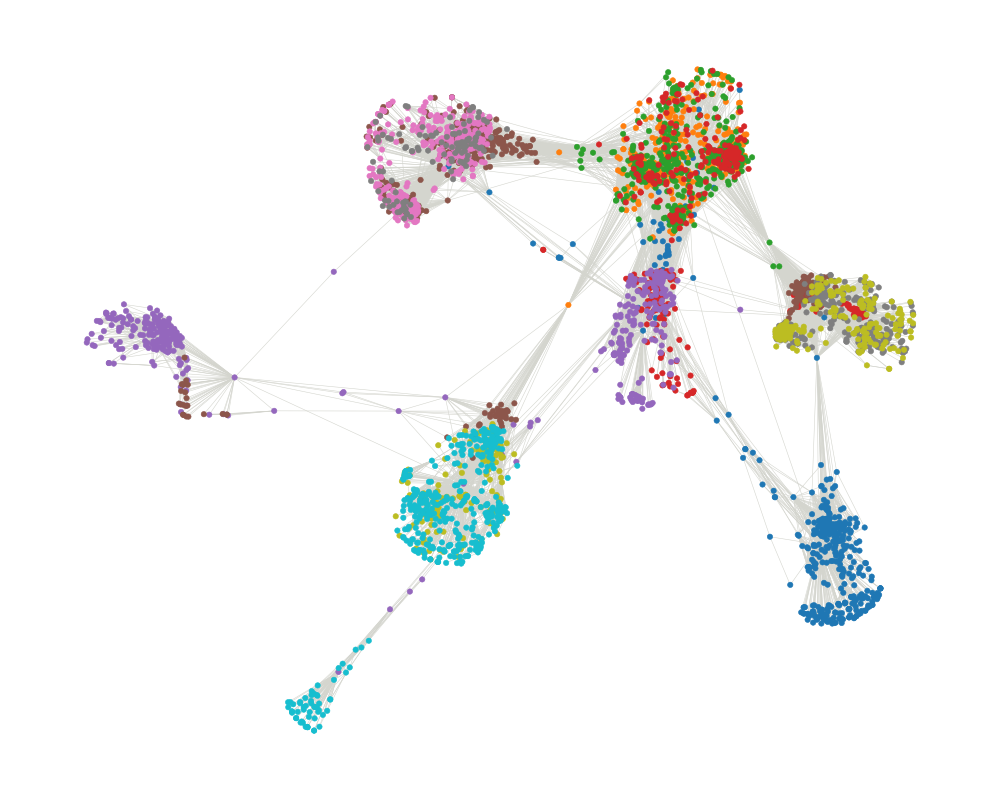
\includegraphics[width=0.7\textwidth]{Graphics/FacebookPoliticalPlot.png}
  \caption{Facebook Graph}
  \label{fig:FacebookGraph}
\end{figure}
\FloatBarrier



Der Graph ähnelt auf den ersten Blick durchaus dem erstellten Plot \ref{fig:SNA}. Sofort fällt aber auf, dass dieser Graph aus deutlich mehr Knoten besteht, zudem weniger Subgraphen aber dennoch im Grunde eine ähnliche Struktur aufweist. Die Berechnungen der Zentralitäten befinden sich auf Github \cite{TZ}. Nun interessiert uns jedoch, wie diese Zentralitäten verteilt sind und ob dieser Graph die erwarteten Verteilungen erfüllen kann. Nachdem wir den Datensatz durch den Code laufen lassen haben, konnten wir folgenden Plot generieren:

\FloatBarrier
\begin{figure}[h!]%
  \centering
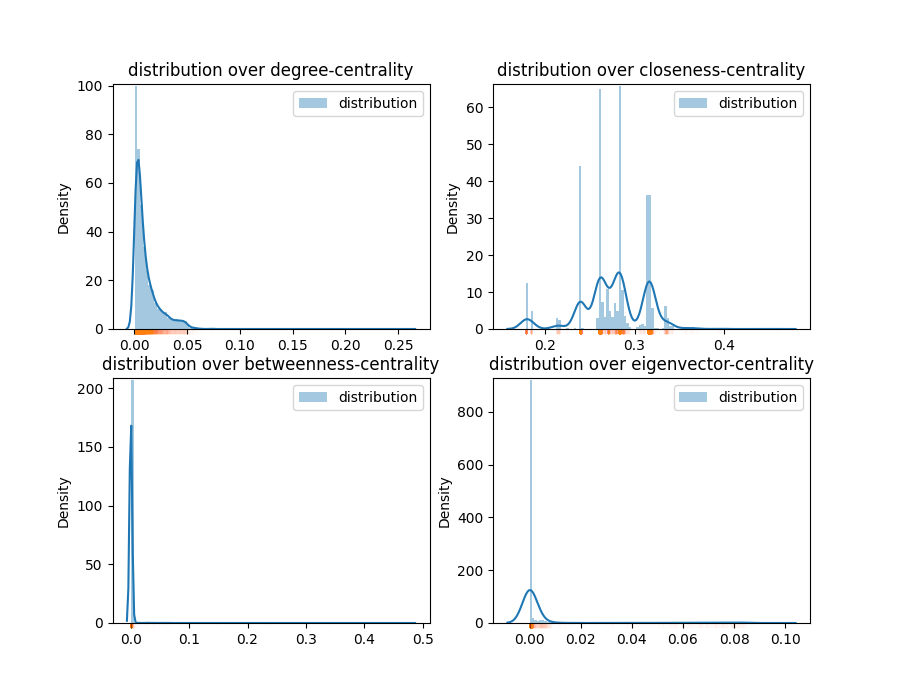
\includegraphics[width=0.8\textwidth]{Graphics/FacebookDistribution.png}
  \caption{Facebook Graph}
  \label{fig:FacebookGraphDistribution}
\end{figure}
\FloatBarrier

Sofort fällt auf, dass wir bei keiner Zentralität eine Normalverteilung sehen. Die \textbf{Grad-Zentralität} fällt uns aber direkt auf, denn es handdelt sich hier um eine Exponentialverteilung. Die anderen Balkendiagramme der \textbf{Betweenness-} und \textbf{Eigenvektor-Zentralität} ähneln jedoch stark den Verteilungen aus \ref{fig:distributionALL}. Was zudem auffällig ist, dass die Diagramm stark an die Verteilungen von \ref{fig:distributionGOT} erinnern. Auch wenn diese Ergebnisse sehr ernüchtern scheinen und vor allem das Balkendiagramm der \textbf{Nähe-Zentralität} sehr eigen. Wir erkennen eine starke Fluktuation der Balken und daher keine schöne Verteilung, die wir aus der Mathematik als Vergleich anbringen könne. Visuell fällt aber  aber visuell auf, dass der Graph \ref{fig:FacebookGraphDistribution} verglichen mit dem Plot des Graphen \ref{ch:SNA} durchaus Parallelen aufweist. Wir sehen deutliche Ansammlungen von Knoten die auch gut als Teilgraphen bezeichnet werden können. Zwischen den Teilgraphen erkenne wir, so wie bei \ref{fig:SNA} einige Kanten, die die Teilgraphen untereinander verbinden. Natürlich weist der obige Graph deutlich mehr Kanten und Knoten auf. Unsere Graphen haben im Schnitt um die \textbf{950} Knoten und \textbf{8700} Kanten, daher also circa neun mal so viele Kanten wie Knoten. Auch haben wir im Schnitt um die \textbf{10100} Cliquen, welche maximal acht Knoten groß sind. Bei dem Facebook Graphen \ref{fig:FacebookGraph} hingegen sprechen wir von \textbf{4093} Knoten und \textbf{88234} Kanten. Das heißt circa einundzwanzig mal so viele Kanten wie Knoten. Doch als wir unsere Kanten und Knoten im Code erhöht haben, um ebenfalls die selbe Relation zu erhalten, waren alle vier untersuchten Zentralitäten annähern Normalverteilt. Was zum einen daran liegt, dass wir letztendlich Graphen wie \ref{fig:GOT2.0} erhalten haben, die noch viel dichter besetzt waren. Wir können festhalten, dass sich die \textbf{Betweenness-} und \textbf{Eigenvektor-Zentralität} bei allen unsersuchten Datensätzen stark zu unseren Verteilungen des künstlich generierten sozialen Netzwerk ähneln. Auch die die \textbf{Nähe-Zentralität} weist stets ähnliche Verteilungen auf, was die Korrektheit des Graphen \ref{fig:SNA} bestätigt. Doch wundert uns nach wie vor die Verteilung der \textbf{Gradzentralität} weshalb wir noch einen letzten Datensatz untersuchen wollen. 


\todo{noch mehr zu Cliquen und Brücken}
\todo{besseren Datensatz}
\todo{Argumentation wie bei mein Graph dann Verteilung wurde als ich ihn noch angepasst hatte}
\todo{Argumentation warum Differenzen}
\todo{Ausblick und Fazit}


%*****************************************
\chapter{Fazit}\label{ch:fazit}
%*****************************************
%*****************************************
\chapter{Anpassungen und Optimierungen}\label{ch:examples}
%*****************************************
%*****************************************
\chapter{Die zweite Interpretation}\label{ch:examples}
%*****************************************
%----------------------------------------------------------------------------------------



%----------------------------------------------------------------------------------------
%	BACKMATTER
%----------------------------------------------------------------------------------------
\appendix
\cleardoublepage

%----------------------------------------------------------------------------------------
%	TEXT WRAPPING ESPECIALLY FOR BIBLIOGRAPHY
%----------------------------------------------------------------------------------------
\setcounter{biburllcpenalty}{7000}
\setcounter{biburlucpenalty}{8000}

%----------------------------------------------------------------------------------------
%	POST-CONTENT THESIS PAGES
%----------------------------------------------------------------------------------------
\cleardoublepage%----------------------------------------------------------------------------------------
%	BIBLIOGRAPHY
%----------------------------------------------------------------------------------------
% work-around to have small caps also here in the headline
% https://tex.stackexchange.com/questions/188126/wrong-header-in-bibliography-classicthesis
% Thanks to Enrico Gregorio

\defbibheading{bibintoc}[\bibname]{%
  \phantomsection
  \manualmark
  \markboth{\spacedlowsmallcaps{#1}}{\spacedlowsmallcaps{#1}}%
  \addtocontents{toc}{\protect\vspace{\beforebibskip}}%
  \addcontentsline{toc}{chapter}{\tocEntry{#1}}%
  \chapter*{#1}%
}
\printbibliography[heading=bibintoc]

\cleardoublepage%----------------------------------------------------------------------------------------
%	DECLARATION
%----------------------------------------------------------------------------------------
\pdfbookmark[0]{Declaration}{declaration}
\begingroup
\let\clearpage\relax
\let\cleardoublepage\relax
\let\cleardoublepage\relax

%----------------------------------------------------------------------------------------
%	GERMAN
%----------------------------------------------------------------------------------------
\begin{otherlanguage}{ngerman}
\pdfbookmark[1]{Erklärung}{Erklärung}
\chapter*{Erklärung}
Hiermit erkläre ich, dass ich die vorliegende Ausarbeitung selbst und ohne Verwendung anderer als der zitierten Quellen und Hilfsmittel verfasst habe. Wörtlich zitierte Sätze oder Satzteile sind als solche kenntlich gemacht; andere Hinweise zur Aussage und zum Umfang sind durch vollständige Angaben zu den betreffenden Publikationen gekennzeichnet. Die Ausarbeitung wurde in gleicher oder ähnlicher Form keiner Prüfungsstelle vorgelegt und ist nicht veröffentlicht worden. Diese Arbeit wurde noch nicht, auch nicht teilweise, in einer anderen Prüfung oder als Lehrveranstaltungsleistung verwendet.
\end{otherlanguage}

\bigskip

%----------------------------------------------------------------------------------------
%	DATE AND SIGNATURE
%----------------------------------------------------------------------------------------
\noindent\textit{\myLocation, \myTime}

\smallskip

\begin{flushright}
    \begin{tabular}{m{5cm}}
        \\ \hline
        \centering\myName \\
    \end{tabular}
\end{flushright}

\endgroup
\vfill

\cleardoublepage\include{FrontBackmatter/Colophon}

%----------------------------------------------------------------------------------------
%	END DOCUMENT
%----------------------------------------------------------------------------------------
\end{document}
% ********************************************************************
